\documentclass[a4paper]{scrreprt}


%% Language and font encodings
\usepackage[german]{babel}
\setcounter{secnumdepth}{3} 
\setcounter{tocdepth}{3} 
\usepackage[utf8x]{inputenc}
\usepackage[T1]{fontenc}
\usepackage{courier}

%% Sets page size and margins
\usepackage[a4paper,top=3cm,bottom=2cm,left=3cm,right=3cm,marginparwidth=1.75cm]{geometry}

%% Useful packages
\usepackage{amsmath}
\usepackage{graphicx}
\usepackage[colorinlistoftodos]{todonotes}
\usepackage[colorlinks=true, allcolors=blue, breaklinks = true]{hyperref}
\usepackage{tocstyle}
\usepackage{longtable}
\usetocstyle{standard}
\settocfeature{raggedhook}{\raggedright}
\usepackage{graphicx}
\usepackage{float}
\graphicspath{ {images/} }

\title{Entwurfsdokument}
\author{Yunjia Chen, Jasmin Jat, Min Hye Park, Alina Shah, Lisa Wang}

\begin{document}
\maketitle
\tableofcontents 
\newpage
\chapter{Einleitung}
Dies ist das Dokument für den Entwurf der Applikation Fridget – entstanden im Rahmen des Softwarepraktikums PSE im Sommersemester 2018.
Es wird zunächst der Grobentwurf vorgestellt, welcher sich in Systemarchitektur, Systemkomponenten und deren Beschreibung unterteilt. 
Der Feinentwurf wird in Abschnitt 3 beschrieben, wobei eine Aufteilung in ``Klassen des Clients'', ``RESTfulAPI'' und ``Klassen des Servers'' erfolgt. Ebenfalls ist ein Klassendiagramm für die Client bzw. Serverseite zu finden. 
Ebenso wichtig ist die Dynamik der Applikation, welche im nachfolgenden Abschnitt 4 in mehreren Sequenz- und Aktivitätsdiagrammen dargestellt und beschrieben wird.  
Im darauf folgenden Abschnitt 5 wird auf die Änderungen zum Pflichtenheft eingegangen und die Begründung für diese Entscheidung erläutert.
Im Anhang ist die Ansicht des gesamten Klassendiagramms zu sehen.
Um Fachbegriffe zu erläutern, befindet sich im letzten Abschnitt ein Glossar.
 

\chapter{Grobentwurf}
	\section{Systemarchitektur}
		Die Applikation Fridget bedient sich der Server-Client Architektur. Es gibt also einen zentralen Server, der als Bindeglied zwischen beliebig vielen Clients fungiert.

Der Server verarbeitet alle Anfragen, die von den unterschiedlichen Clients gestellt werden. Er verwaltet die Datenbank und stellt alle Daten bereit, worauf die Clients zugreifen können.

Jeder Benutzer, welches die Applikation Fridget benutzt, hat einen festen User-ID, der lokal auf dem Gerät gespeichert wird. Damit stellt jeder Benutzer ein Client dar, welcher mit seiner User-ID Anfragen an den Server schicken kann. 
Die Architektur der einzelnen Seiten wird im folgenden beschrieben.  

		\subsection{MVVM}
			Für die Client-Seite verwenden wir das MVVM (Model-View-View-Model) Architektur-Muster mit Datenbindung. 
Dabei wird die Darstellung in View, die Eingabeverarbeitung in View Model und die Datenhaltung in Model aufgeteilt. Zusätzlich dient der Service noch als direkten Vermittler zwischen der Client- und Server-Seite.

Dieses Muster hat zwei wesentliche Vorteile.

Erstens, es gibt keine Abhängigkeit zwischen der View und dem Model. Die Daten, die für die View benötigt werden, werden nämlich im ViewModel bereitgestellt.

Zweitens, das ViewModel ist nicht von der View abhängig. Durch Data Binding kann ohne Referenz auf die View der Zustand der View im ViewModel verwaltet werden. 

Es ist also eine lose Kopplung vorhanden, welches die Testbarkeit verbessert.

		\subsection{MVC}
			Auf der Server-Seite wird das MVC (Model-View-Controller) Architektur-Muster eingesetzt. Dabei ist in unserem Falle die Client-Seite die View. Model ist für die Datenhaltung zuständig und der Controller steuert zwischen View, Model sowie Repository.  
Sobald auf Client-Seite eine Interaktion mit dem Benutzer und der Applikation geschieht, wird dies vom Service der Client-Seite weiter an dem Controller geleitet. Dieser kann die Veränderungen dann durchführen lassen.
Gleichzeitig beobachtet die Client-Seite die Server-Seite, sodass Veränderungen sofort von allen Clients übernommen werden kann.

		
	\section{Systemkomponenten}
	      \begin{figure}[H]
	       \centering
	       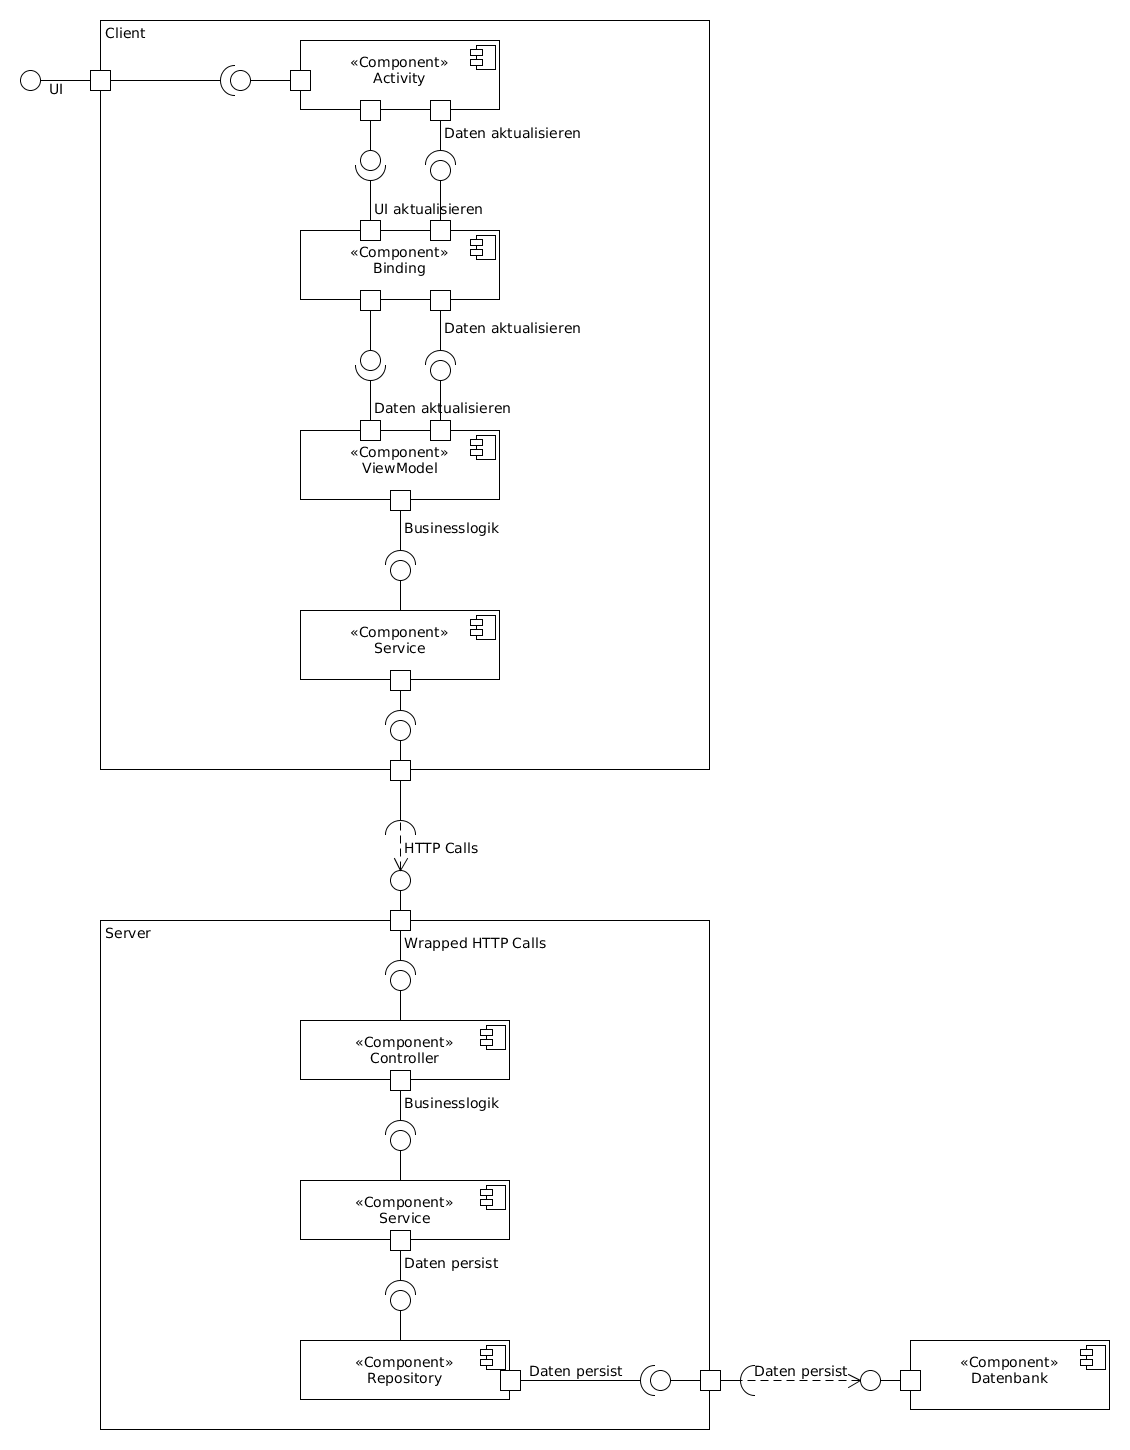
\includegraphics[scale = .35]{systemkomponenten.png}
	       \caption{Systemkomponenten}
	      \end{figure}
      
      \newpage
	 
	 \section{Komponentenbeschreibung}
		 \subsection{Client}
	 		\subsubsection{MVVM-Architektur}

\textbf{Model}\\
Model-Klassen kapseln die Appdaten ab. Es handelt sich um eine Datenzugriffschicht, wo die Daten gehalten und zum Benutzen aufbereitet werden.


\textbf{View}\\
Zu jeder Activity gehört eine View, die als graphische Benutzeroberfläche dient. Sie stellt eine rechteckige Fläche auf dem Bildschirm dar und ist verantwortlich fürs Event-Handling. Die View ist das, was der Benutzer sieht und mit dem er interagieren kann (Buttons, Textfelder, etc.).


\textbf{Viewmodel}\\
Viewmodel definiert die in der View angezeigten Inhalte und dient zur Eingabeverarbeitung. Sie kümmern sich darum, Eigenschaften und Befehle zu implementieren und tauscht mit der View mittels Data Binding Daten aus. Außerdem sind Viewmodels dafür verantwortlich, die Views mittels Live Data über Zustandsänderungen zu benachrichtigen. Viewmodels kümmern sich also um die Geschäftslogik, die von den Views verwendet und angezeigt wird.


\subsubsection{}   \todo{Überschriften finden}
\textbf{Activity}\\
Die Activities stellen die Benutzerschnittstelle unserer App dar und kümmern sich um die Interaktionen mit unserer Benutzeroberfläche. In jeder Activity-Klasse befinden sich selbstverständlich die üblichen Methoden eines Activity-Lifecycles: onCreate() zum Erstellen, onStart() zum Starten, onPause() zum Pausieren , onResume() zum Fortsetzen, onStop() zum Stoppen und onDestroy() zum Zerstören der Activity.

\subsubsection{} \todo{Überschriften finden}
\textbf{Service}\\
Ein Dienst ist eine Komponente, die ohne direkte Interaktion mit dem Benutzer im Hintergrund abläuft. Da der Service keine Benutzeroberfläche hat, ist er nicht an den Lebenszyklus einer Aktivität gebunden.
Jede Methode innerhalb einer Service- Schnittstelle repräsentiert einen möglichen API-Aufruf. Es muss eine HTTP-Annotation (GET, POST usw.) haben, um den Anforderungstyp und die relative URL anzugeben. Der Rückgabewert umschließt die Antwort in einem Call-Objekt mit dem Typ des erwarteten Ergebnisses.


\subsubsection{} \todo{Überschriften finden}
\textbf{Live-Data}\\
Live-Data sind beobachtbare data holder Klassen. Live-Data ist wie der Observer-Entwurfsmuster. Sie benachrichtigt den Observer-Objekt, in unserem Fall die View, wenn sich die Objekte verändern. 

\subsubsection{} \todo{Überschriften finden}
\textbf{Retrofit}\\
Retrofit ist ein typsicherer HTTP-Client für Android und Java. Es ist eine Open-Source-Bibliothek, die die HTTP-Kommunikation vereinfacht, indem MRemote-APIs zu deklarativen, typsicheren Schnittstellen werden. Es macht es relativ einfach, JSON (oder andere strukturierte Daten) über einen REST-basierten Webservice abzurufen und hochzuladen. Es serialisiert die JSON-Antwort automatisch unter Verwendung eines POJO(Plain Old Java Object), das für die JSON-Struktur im Voraus definiert werden muss.


\subsubsection{} \todo{Überschriften finden}
\textbf{REST-Client}\\
Der REST-Client unserem Fall die Retrofit-Bibliothek, die auf der Clientseite (Android) verwendet wird, um eine HTTP-Anforderung an die REST-API zu stellen.

\textbf{REST-API}\\
Die REST-API definiert eine Reihe von Funktionen, mit denen Entwickler Anfragen ausführen und Antworten über HTTP-Protokoll wie GET und POST empfangen können.

	 		
	 	 \subsection{REST-API}
	 	 	Die REST-API definiert eine Reihe von Funktionen, mit denen Entwickler Anfragen ausführen und Antworten über HTTP-Protokoll wie GET und POST empfangen können.
	 	 	
	  \newpage
		
		 \subsection{Server}
	 	 	
\subsubsection{MVC-Architektur}

\textbf{Model} \\
Das Model enthält Daten, die vom Controller gespeichert, geladen und geändert werden und vom View dargestellt werden. 

\textbf{View}\\



\textbf{Controller}\\
Der Controller verwaltet den View und das Model. In unserem Fall implementiert der Controller eine REST-API, behandelt HTTP-Anfrage und gibt HTTP-Antwort zurück.


\textbf{Service}\\
Die Service-Schicht trennt die Businesslogik aus dem Controller und behandelt spezifische Transaktionsverhalten.

\textbf{Repository}\\ 
Die Repository-Schicht ist die unterste Schicht in unserer App. Es reduziert den erforderlichen Code für die Implementierung von DAO (Data Access Object) für Persistenz. Unsere Repositories erweitern das JpaRepository, bieten CRUD-Funktionen und JPA-relevante Methoden an.

 \subsubsection{Framework}

\textbf{Spring Boot mit JPA und Hibernate}
Für unsere RESTful Services verwenden wir Spring Boot mit JPA und Hibernate. 
Spring Boot erleichtert die Entwicklung der Anwendungen per Convention over Configuration. Mit Hilfe einfacher Annotationen wird einen embedded Tomcat Webserver integriert, der REST-Services anbietet.
Die JPA (Java Persistence API) ist eine Schnittstelle für Java-Anwendungen, die die Zuordnung und die Übertragung von Objekten zu Datenbankeinträgen vereinfacht.
Hibernate ist ein Persistenz- und O-R-Mapping-Framework für Java. Das ermöglicht es, POJOs in relationalen Datenbanken (MySQL in unserem Fall) zu speichern und aus entsprechenden Datensätzen wiederum Objekte zu erzeugen.

\subsubsection{Datenbank}
\textbf{MySQL}
MySQL ist eine der am häufigsten benutzte, zuverlässige relationale Datenbank. Sie beruht auf dem relationalen Datenbankmodell und speichert Daten in verschiedenen Tabellen, die untereinander verknüpft werden. 

	 	 
        
\newpage

\chapter{Feinentwurf}
	\section{Klassen des Clients}
	\subsection{Klassendiagramm}
	\begin{figure}[H]
	       \centering
	       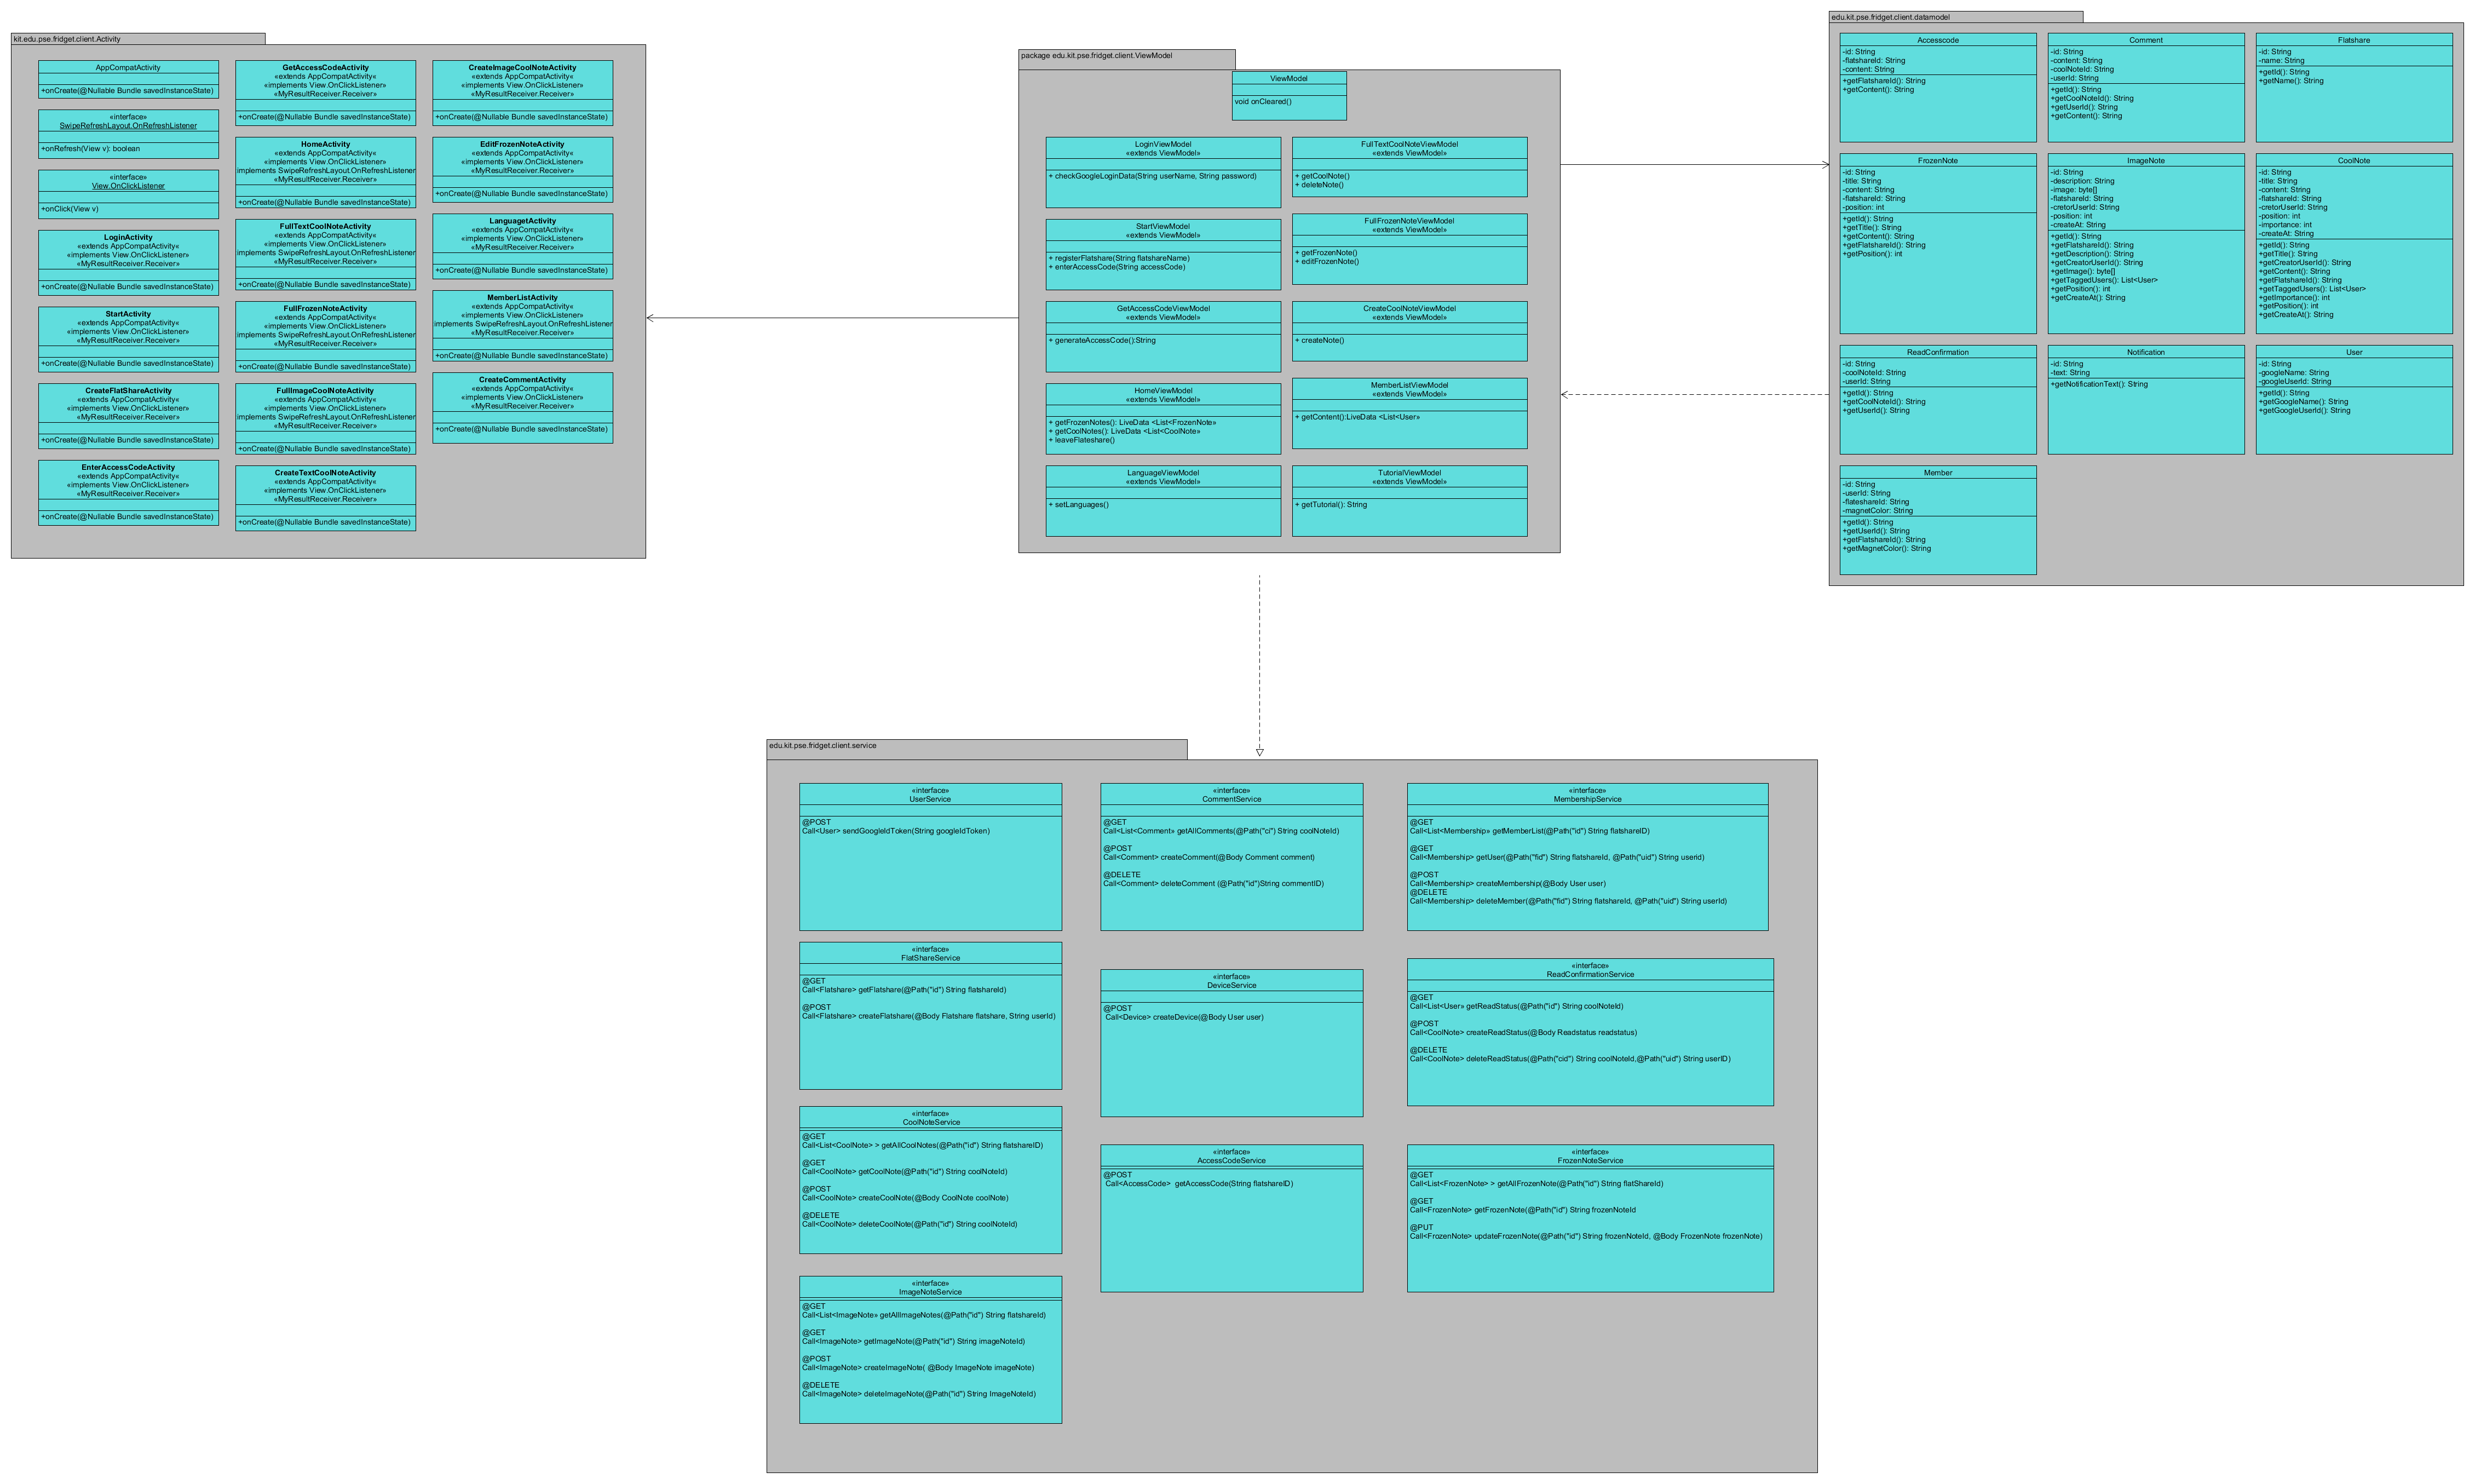
\includegraphics[scale = .11]{all_client_packages.png}
	       \caption{Klassen des Clients}
	      \end{figure}
	
	\subsection{package kit.edu.pse.fridget.client.activity}
\begin{figure}[H]
	       \centering
	       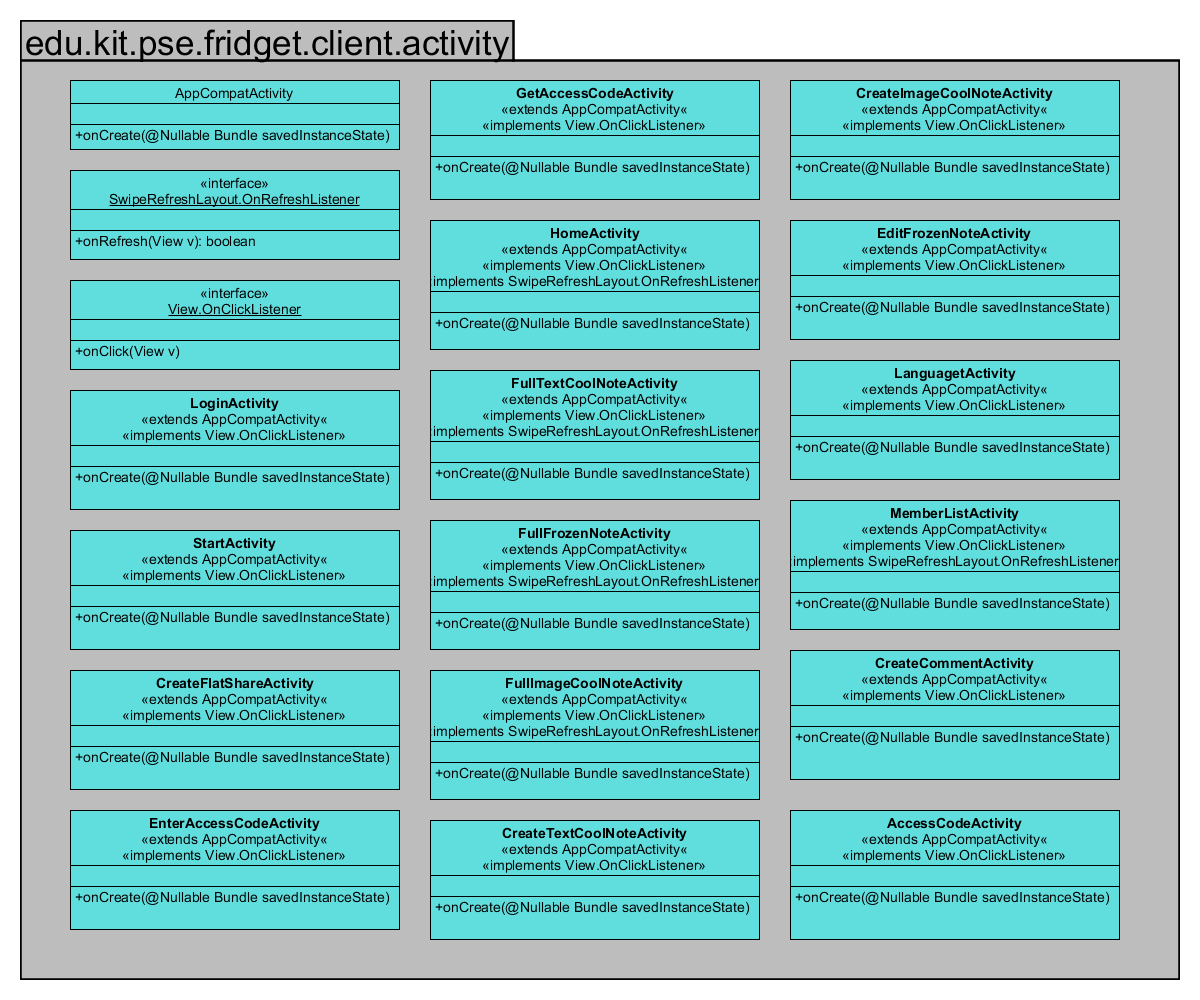
\includegraphics[scale = .35]{klassendiagramm_activity.png}
	       \caption{Klassen der Activities}
	      \end{figure}
\subsubsection{\texttt{public class AppCompatActivity}}

Unsere App setzt sich aus 16 Activites zusammen.\\

	\textbf{Beschreibung} \\
	\textit{Basisklasse für alle Activities} \\

	\textbf{Methoden}
	\begin{itemize}
		\item{\texttt{public void onCreate(@Nullable Bundle savedInstanceState)}}\\
	\textit{Hier wird das Layout der Activity erstellt.}\\
	\end{itemize}

	\textbf{Parameter}
	\begin{itemize}
		\item\texttt{Bundle savedInstanceState}\\ 
	\textit{Die zuvor gespeicherte Instanz der Activity, die wieder hergestellt zwird, sonst NULL}\\
	\end{itemize}

\subsubsection{\texttt{public static interface View.OnClickListener}}

	\textbf{Beschreibung} \\
	\textit{Schnittstelle dafür, wenn auf die View geklickt wird.klickt wird.}\\

	\textbf{Methoden}
	\begin{itemize}
	\item{\texttt{public void onClick(View v)}}\\
	\textit{Aufruf bei einen Klick auf ein Element.}\\
	\end{itemize}

	\textbf{Parameter}
	\begin{itemize}
	\item\texttt{View v}\\
	\textit{Die angeklickte View}\\
	\end{itemize} 

\subsubsection{\texttt{public static interface SwipeRefreshLayout.OnRefreshListener}}

	\textbf{Beschreibung} \\
	\textit{Schnittstelle dafür, wenn durch Hinunter-Swipen eine Aktualisierung ausgeführt werden soll} \\

	\textbf{Methoden}
	\begin{itemize}
		\item\texttt{{public boolean onRefresh()}}\\
	\textit{Aufruf beim Hinunter-Swipen zum Aktualisieren}\\
	\end{itemize}       

\subsubsection{\texttt{public class LoginActivity extends AppCompatActivity implements View.OnClickListener}}

	\textbf{Beschreibung} \\
	\textit{Diese Klasse zeigt den Login mit dem Google-Account. Man kann seinen Google-Account-Daten eingeben und sich anmelden.} \\

	\textbf{Methoden}
	\begin{itemize}
		\item\texttt{{public void onCreate(@Nullable Bundle savedInstanceState)}}\\
	\textit{Hier wird das Layout der Activity erstellt.}\\
	\end{itemize}

	\textbf{Parameter}
	\begin{itemize}
		\item\texttt{Bundle savedInstanceState}\\ 
	\textit{Die zuvor gespeicherte Instanz der Activity, die wieder hergestellt zwird, sonst NULL}\\
	\end{itemize}

\subsubsection{\texttt{public class StartActivity extends AppCompatActivity implements View.OnClickListener}}

	\textbf{Beschreibung} \\
	\textit{Diese Klasse zeigt den Startbildschirm mit dem App-Logo und zwei Buttons: Ein Button zum Erstellen einer WG und einer zum Eingeben eines Zugangscodes.} \\

	\textbf{Methoden}
	\begin{itemize}
		\item\texttt{{public void onCreate(@Nullable Bundle savedInstanceState)}}\\
	\textit{Hier wird das Layout der Activity erstellt.}\\
	\end{itemize}

	\textbf{Parameter}
	\begin{itemize}
		\item\texttt{Bundle savedInstanceState}\\ 
	\textit{Die zuvor gespeicherte Instanz der Activity, die wieder hergestellt zwird, sonst NULL}\\
	\end{itemize}       

\subsubsection{\texttt{public class CreateFlatshareActivity extends AppCompatActivity implements View.OnClickListener}}

	\textbf{Beschreibung} \\
	\textit{In dieser Klasse kann man der WG einen Namen geben und kann mithilfe eines Buttons zur HomeActivity gelangen.} \\

	\textbf{Methoden}
	\begin{itemize}
		\item\texttt{{public void onCreate(@Nullable Bundle savedInstanceState)}}\\
	\textit{Hier wird das Layout der Activity erstellt.}\\
	\end{itemize}

	\textbf{Parameter}
	\begin{itemize}
		\item\texttt{Bundle savedInstanceState}\\ 
	\textit{Die zuvor gespeicherte Instanz der Activity, die wieder hergestellt zwird, sonst NULL}\\
	\end{itemize}      

\subsubsection{\texttt{public class GetAccessCodeActivity extends AppCompatActivity implements View.OnClickListener}}

	\textbf{Beschreibung} \\
	\textit{In dieser Klasse kriegt man den Zugangscode und kann mithilfe eines Buttons zur HomeActivity gelangen.} \\

	\textbf{Methoden}
	\begin{itemize}
		\item\texttt{{public void onCreate(@Nullable Bundle savedInstanceState)}}\\
	\textit{Hier wird das Layout der Activity erstellt.}\\
	\end{itemize}

	\textbf{Parameter}
	\begin{itemize}
		\item\texttt{Bundle savedInstanceState}\\  
	\textit{Die zuvor gespeicherte Instanz der Activity, die wieder hergestellt zwird, sonst NULL}\\
	\end{itemize}  

\subsubsection{\texttt{public class EnterAccessCodeActivity extends AppCompatActivity implements View.OnClickListener}}

	\textbf{Beschreibung} \\
	\textit{In dieser Klasse kann man den Zugangscode eingeben und kann mithilfe eines Buttons zur HomeActivity gelangen.} \\

	\textbf{Methoden}
	\begin{itemize}
		\item\texttt{{public void onCreate(@Nullable Bundle savedInstanceState)}}\\
	\textit{Hier wird das Layout der Activity erstellt.}\\
	\end{itemize}

	\textbf{Parameter}
	\begin{itemize}
		\item\texttt{Bundle savedInstanceState}\\ 
	\textit{Die zuvor gespeicherte Instanz der Activity, die wieder hergestellt zwird, sonst NULL}\\
	\end{itemize} 

\subsubsection{\texttt{public class HomeActivity extends AppCompatActivity implements View.OnClickListener implements SwipeRefreshLayout.OnRefreshListener}}

	\textbf{Beschreibung} \\
	\textit{Diese Klasse zeigt das View der WG-Pinnwand, man sieht die Notes mit Überschrift und Magnet und einige Buttons. Drei Frozen Notes sind von Anfang an enthalten. Frozen Notes haben immer einen schwarzen Magneten.} \\

	\textbf{Methoden}
	\begin{itemize}
		\item\texttt{{public void onCreate(@Nullable Bundle savedInstanceState)}}\\
	\textit{Hier wird das Layout der Activity erstellt.}\\
	\end{itemize}

	\textbf{Parameter}
	\begin{itemize}
		\item\texttt{Bundle savedInstanceState}\\  
	\textit{Die zuvor gespeicherte Instanz der Activity, die wieder hergestellt zwird, sonst NULL}\\
	\end{itemize} 

\subsubsection{\texttt{public class FullTextCoolNoteActivity extends AppCompatActivity implements View.OnClickListener implements SwipeRefreshLayout.OnRefreshListener}}

	\textbf{Beschreibung} \\
	\textit{Diese Klasse zeigt eine Großansicht einer Text-Cool-Note mit zugehörigem Magneten, Erstelldatum, Tags, Titel, Inhalt, Lesebestätigungen und Kommentaren. Der @All-Tag ist immer da, wenn keine Tags spezifiziert werden. Es stehen wieder einige Buttons zur Interaktion zu Verfügung.} \\

	\textbf{Methoden}
	\begin{itemize}
		\item\texttt{{public void onCreate(@Nullable Bundle savedInstanceState)}}\\
	\textit{Hier wird das Layout der Activity erstellt.}\\
	\end{itemize}

	\textbf{Parameter}
	\begin{itemize}
		\item\texttt{Bundle savedInstanceState}\\ 
	\textit{Die zuvor gespeicherte Instanz der Activity, die wieder hergestellt zwird, sonst NULL}\\
	\end{itemize} 

\subsubsection{\texttt{public class FullFrozenNoteActivity extends AppCompatActivity implements View.OnClickListener implements SwipeRefreshLayout.OnRefreshListener}}

	\textbf{Beschreibung} \\
	\textit{Diese Klasse zeigt eine Großansicht einer Frozen Note mit zugehörigem schwarzen Magneten, Titel und Inhalt. Es stehen wieder einige Buttons zur Interaktion zu Verfügung.} \\

	\textbf{Methoden}
	\begin{itemize}
		\item\texttt{{public void onCreate(@Nullable Bundle savedInstanceState)}}\\
	\textit{Hier wird das Layout der Activity erstellt.}\\
	\end{itemize}

	\textbf{Parameter}
	\begin{itemize}
		\item\texttt{Bundle savedInstanceState}\\ 
	\textit{Die zuvor gespeicherte Instanz der Activity, die wieder hergestellt zwird, sonst NULL}\\
	\end{itemize} 

\subsubsection{\texttt{public class FullImageCoolNoteActivity extends AppCompatActivity implements View.OnClickListener implements SwipeRefreshLayout.OnRefreshListener}}

	\textbf{Beschreibung} \\
	\textit{Diese Klasse zeigt eine Großansicht einer Bild-Cool-Note mit zugehörigem Magneten, Erstelldatum, Tags, Titel, Inhalt, Lesebestätigungen und Kommentaren. Der @All-Tag ist immer da, wenn keine Tags spezifiziert werden. Es stehen wieder einige Buttons zur Interaktion zu Verfügung.} \\

	\textbf{Methoden}
	\begin{itemize}
		\item\texttt{{public void onCreate(@Nullable Bundle savedInstanceState)}}\\
	\textit{Hier wird das Layout der Activity erstellt.}\\
	\end{itemize}

	\textbf{Parameter}
	\begin{itemize}
		\item\texttt{Bundle savedInstanceState}\\ 
	\textit{Die zuvor gespeicherte Instanz der Activity, die wieder hergestellt zwird, sonst NULL}\\
	\end{itemize} 

\subsubsection{\texttt{public class CreateTextCoolNoteActivity extends AppCompatActivity implements View.OnClickListener}}

	\textbf{Beschreibung} \\
	\textit{Diese Klasse zeigt das View für die Erstellung einer Text-Cool-Note. Dieses View wird auch für die Kommentar-Funktion benutzt, nur, dass man keinen Titel schreiben und keine Wichtigkeit auswählen kann. Das View öffnet sich auch, wenn man eine Frozen Note editieren will, wobei die Wichtigkeit wieder nicht auswählbar ist.} \\

	\textbf{Methoden}
	\begin{itemize}
		\item\texttt{{public void onCreate(@Nullable Bundle savedInstanceState)}}\\
	\textit{Hier wird das Layout der Activity erstellt.}\\
	\end{itemize}

	\textbf{Parameter}
	\begin{itemize}
		\item\texttt{Bundle savedInstanceState}\\  
	\textit{Die zuvor gespeicherte Instanz der Activity, die wieder hergestellt zwird, sonst NULL}\\
	\end{itemize} 


\subsubsection{\texttt{public class CreateImageCoolNoteActivity extends AppCompatActivity implements View.OnClickListener}}

	\textbf{Beschreibung} \\
	\textit{Diese Klasse zeigt das View für die Erstellung einer Bild-Cool-Note.} \\

	\textbf{Methoden}
	\begin{itemize}
		\item\texttt{{public void onCreate(@Nullable Bundle savedInstanceState)}}\\
	\textit{Hier wird das Layout der Activity erstellt.}\\
	\end{itemize}

	\textbf{Parameter}
	\begin{itemize}
		\item\texttt{Bundle savedInstanceState}\\ 
	\textit{Die zuvor gespeicherte Instanz der Activity, die wieder hergestellt zwird, sonst NULL}\\
	\end{itemize} 

\subsubsection{\texttt{public class CreateCommentActivity extends AppCompatActivity implements View.OnClickListener}}

	\textbf{Beschreibung} \\
	\textit{Diese Klasse zeigt das View für die Erstellung eines Kommentars.} \\

	\textbf{Methoden}
	\begin{itemize}
		\item\texttt{{public void onCreate(@Nullable Bundle savedInstanceState)}}\\
	\textit{Hier wird das Layout der Activity erstellt.}\\
	\end{itemize}

	\textbf{Parameter}
	\begin{itemize}
		\item\texttt{Bundle savedInstanceState}\\  
	\textit{Die zuvor gespeicherte Instanz der Activity, die wieder hergestellt zwird, sonst NULL}\\
	\end{itemize} 


\subsubsection{\texttt{public class EditFrozenNoteActivity extends AppCompatActivity implements View.OnClickListener}}

	\textbf{Beschreibung} \\
	\textit{Diese Klasse zeigt das View für die Bearbeitung einer Frozen Note.} \\

	\textbf{Methoden}
	\begin{itemize}
		\item\texttt{{public void onCreate(@Nullable Bundle savedInstanceState)}}\\
	\textit{Hier wird das Layout der Activity erstellt.}\\
	\end{itemize}

	\textbf{Parameter}
	\begin{itemize}
		\item\texttt{Bundle savedInstanceState}\\ 
	\textit{Die zuvor gespeicherte Instanz der Activity, die wieder hergestellt zwird, sonst NULL}\\
	\end{itemize} 

\subsubsection{\texttt{public class MemberListActivity extends AppCompatActivity implements View.OnClickListener implements SwipeRefreshLayout.OnRefreshListener}}

	\textbf{Beschreibung} \\
	\textit{Diese Klasse zeigt das View zum Einsehen der aktuellen Mitglieder mit
mit zugehörigem Magneten.} \\

	\textbf{Methoden}
	\begin{itemize}
		\item\texttt{{public void onCreate(@Nullable Bundle savedInstanceState)}}\\
	\textit{Hier wird das Layout der Activity erstellt.}\\
	\end{itemize}

	\textbf{Parameter}
	\begin{itemize}
		\item\texttt{Bundle savedInstanceState}\\  
	\textit{Die zuvor gespeicherte Instanz der Activity, die wieder hergestellt zwird, sonst NULL}\\
	\end{itemize} 

\subsubsection{\texttt{public class LanguageActivity extends AppCompatActivity implements View.OnClickListener}}

	\textbf{Beschreibung} \\
	\textit{Diese Klasse zeigt das View zum Einstellen der App-Sprache.} \\

	\textbf{Methoden}
	\begin{itemize}
		\item\texttt{{public void onCreate(@Nullable Bundle savedInstanceState)}}\\
	\textit{Hier wird das Layout der Activity erstellt.}\\
	\end{itemize}

	\textbf{Parameter}
	\begin{itemize}
		\item\texttt{Bundle savedInstanceState}\\  
	\textit{Die zuvor gespeicherte Instanz der Activity, die wieder hergestellt zwird, sonst NULL}\\
	\end{itemize} 

\subsubsection{\texttt{public class AccessCodeActivity extends AppCompatActivity implements View.OnClickListener}}

\textbf{Beschreibung} \\
\textit{Diese Klasse zeigt das View zum Erstellen eines neuen Zugangscodes.} \\

\textbf{Methoden}
\begin{itemize}
	\item\texttt{{public void onCreate(@Nullable Bundle savedInstanceState)}}\\
	\textit{Hier wird das Layout der Activity erstellt.}\\
\end{itemize}

\textbf{Parameter}
\begin{itemize}
	\item\texttt{Bundle savedInstanceState}\\  
	\textit{Die zuvor gespeicherte Instanz der Activity, die wieder hergestellt zwird, sonst NULL}\\
\end{itemize} 

\newpage

	    
	\clearpage
			\subsection{package kit.edu.pse.fridget.client.viewmodel}
		\begin{figure}[H]
	       \centering
	       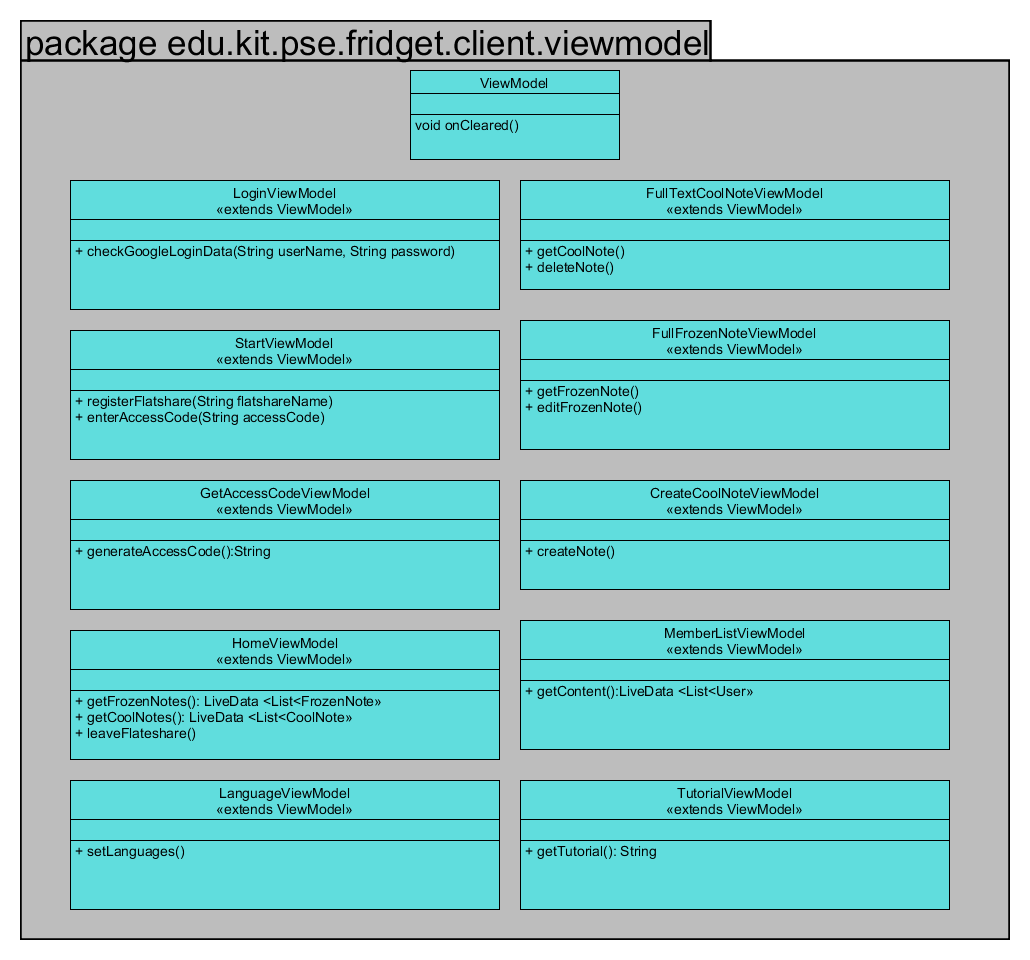
\includegraphics[scale = .35]{ViewModel.png}
	       \caption{Klassen des ViewModels}
	      \end{figure}
		\subsubsection{\texttt{public class LoginViewModel extends ViewModel}}
        \textit{LoginViewModel ist das ViewModel zur LoginActivity. In dieser Klasse wird geprüft, ob der Benutzer sich korrekt einloggt.}\\
        
		\textbf{Methoden} \\
 			\begin{itemize}
        		\item{public void checkGoogleLoginData(String userName, String password)}
        	
        		\textit{Diese Methode überprüft ob die eingegebenen Google-Daten richtig sind}
        	
        		\textbf{Parameter} \\
				userName: Google-Account Adresse

				\textbf{Parameter} \\
				password: Passwort

				\textbf{Rückgabewert} \\
				boolean: gibt an, ob die eingebenen Werte richtig oder falsch sind
   
       		 \end{itemize}
             
             	\subsubsection{\texttt{StartViewModel extends ViewModel}}
        \textit{Diese Klasse ist das ViewModel zur StartActivity, CreateFlatshareActivity, EnterAccessCodeActivity. Sie ermöglicht das Einloggen in die WG und stellt alle Daten der WG zur Verfügung.}\\
        \\
		\textbf{Methoden} \\
 			\begin{itemize}
        		\item{public void registerFlatshare(String flatshareName)}
        	
        		\textit{Diese Methode lässt eine neue WG mit dem übergebenen Namen erstellen. Dabei erstellt sie ein Objekt des Models User und übergibt diesen dem FlatShareService. Wenn in der Datenbank eine neue Flatshare angelegt wurde, erfragt diese Methode die Flatshare-ID und speichert auf einem Local Repository die FlateShare-ID sowie die User-ID.}
        	
        		\textbf{Parameter} \\
				flatshareName: Name der WG


        		\item{public void enterAccessCode(String accessCode)}
        	
        		\textit{Diese Methode lässt den AccessCode überprüfen und stellt die passenden Daten zu der WG bereit. Sobald die FlateShare-ID bekannt ist, wird sie mit der User-ID auf einem Local Repository gespeichert.}
        	
        		\textbf{Parameter} \\
				accessCode: Zugangscode
   
       		 \end{itemize}
             
             		\subsubsection{\texttt{public class GetAccessCodeViewModel extends ViewModel}}
        \textit{Diese Klasse ist das ViewModel zur GetAccessCodeActivity. Sie dient zur Generierung des Zugangscodes.}\\
        \\
		\textbf{Methoden} \\
 			\begin{itemize}
        		\item{public String generateAccessCode()}
        	
        		\textit{Diese Methode lässt einen zufälligen, einzigartigen AccessCode generieren und gibt diesen zurück.}
        	
        		\textbf{Rückgabewert} \\
				Der generierte Zugangscode wird zurückgegeben.
   
       		 \end{itemize}
             
             
            		\subsubsection{\texttt{public class HomeViewModel extends ViewModel}}
        \textit{HomeViewModel ist das ViewModel zur HomeActivity. Diese Klasse aktualisiert die Daten in der HomeActivity. Sie überprüft also, ob die Anordnung der Cool Notes verändert wurde, ob die Frozen Notes verändert wurden usw.}\\      
        \\
		\textbf{Methoden} \\
 			\begin{itemize}
        		\item{public LiveData <List<FrozenNote>> getFrozenNotes()}
        	
        		\textit{Diese Methode übergibt die Daten aller Frozen Notes auf der Pinnwand.}
        		
        		\textbf{Rückgabewert} \\
				Die Liste an Frozen Notes wird in Form von LiveData zurückgegeben.
        	
        		\item{public LiveData <List<CoolNote>> getCoolNotes()}

        		\textit{Diese Methode holt sich die Daten aller Cool Notes auf der Pinnwand sowie deren Anordnung.}
        		
        		\textbf{Rückgabewert} \\
				Die Liste an Cool Notes wird in Form von LiveData zurückgegeben.
				
				\item{public void leaveFlateshare()}
        	
        		\textit{Diese Methode sorgt dafür, dass alles, was derjenige, der die WG verlässt, erstellt hat, gelöscht wird. Außerdem wird derjenige aus der Mitgliederliste gelöscht.}
        		
       		 \end{itemize}
             
             
           		\subsubsection{\texttt{public class FullTextCoolNoteViewModel extends ViewModel}}
        \textit{Diese Klasse ist das ViewModel zur FullTextCoolNoteActivity und FullImageCoolNoteActivity. Diese Klasse verwaltet alle Daten, die für die Großansicht der Cool Note benötigt wird.}\\
        \\
		\textbf{Methoden} \\
 			\begin{itemize}
        		\item{public void getCoolNote()}
        	
        		\textit{Diese Methode holt alle Daten der CoolNote und speichert sie in einzelne Attribute, die mit den get-Methoden geholt werden können.}
        		
        		\item{public void deleteNote()}
        	
        		\textit{Diese Methode veranlasst das Löschen der Note in der Datenbank.}

       		 \end{itemize}
             
             
                 \subsubsection{\texttt{public class FullFrozenNoteViewModel extends ViewModel}}
        \textit{Diese Klasse ist das ViewModel zur FullTextFrozenNoteActivity. Dieses ViewModel holt alle benötigten Daten für die Großansicht der Frozen Note.}\\
        \\
		\textbf{Methoden} \\
 			\begin{itemize}
        		\item{public void getFrozenNote()}
        	
        		\textit{Diese Methode holt alle Daten der Frozen Note und speichert sie in einzelne Attribute, die mit den get-Methoden geholt werden können.}
        	
        		\item{public void editFrozenNote(String title, String content)}
        	
        		\textit{Diese Methode speichert die neuen Daten.}
        	
        	\textbf{Parameter} \\
				title: Überschrift
				
			\textbf{Parameter} \\
			content: Inhalt
				
       		 \end{itemize}
       		 
           		\subsubsection{\texttt{public class CreateCoolNoteViewModel extends ViewModel}}
        \textit{CreateCoolNoteViewModel ist das ViewModel zur CreateTextCoolNoteActivity und CreateImageCoolNoteActivity. Es wird benötigt, um die neu erstellten Cool Notes zu speichern.}\\
        \\
		\textbf{Methoden} \\
 			\begin{itemize}
        		\item{public void createNote()}
        	
        		\textit{Es wird ein neues Objekt CoolNote erstellt und dem passenden Service übergeben, um die CoolNote in der Datenbank hinzuzufügen. Es wird eine zufällige Position berechnet.}
        	
       		 \end{itemize}
       		 
           		\subsubsection{\texttt{public class MemberListViewModel extends ViewModel}}
        \textit{Diese Klasse ist das ViewModel zur MemberListActivity. Es holt alle Daten bezüglich der Mitglieder. d.h. Magnetfarben und Namen.}\\
        \\
		\textbf{Methoden} \\
 			\begin{itemize}
        		\item{public LiveData <List<User>> getContent()}
        	
        		\textit{Diese Methode gibt die Liste der Mitglieder zurück.}
        	
        	\textbf{Rückgabewert} \\
				Die Liste der Mitglieder wird in Form von LiveData zurückgegeben.
				
       		 \end{itemize}
       		 
       		   \subsubsection{\texttt{public class LanguageViewModel extends ViewModel}}
        \textit{Diese Klasse ist das ViewModel zur LanguageActivity.}\\
        \\
		\textbf{Methoden} \\
 			\begin{itemize}
        		\item{public void setLanguages()}
        	
        		\textit{Diese Methode ändert die Sprache der App.}
        	
       		 \end{itemize}
       		 
           		\subsubsection{\texttt{public class TutorialViewModel extends ViewModel}}
        \textit{Diese Klasse ist das ViewModel zur TutorialActivity.}\\
        \\
		\textbf{Methoden} \\
 			\begin{itemize}
        		\item{public String getTutorial()}
        		
        		\textit{Diese Methode stellt die Daten der Textinhalte zur Verfügung.}
        	
       		 \end{itemize}
	\clearpage
	\subsection{package edu.kit.pse.fridget.client.datamodel}
\subsubsection{\texttt{public class Accesscode}}

	\textbf{Beschreibung} \\
	\textit{Die Klasse Accesscode stellt der Access-Code, oder Zugangscode einer WG dar.} \\

	\textbf{Methoden}
	\begin{itemize}
		\item{\texttt{public String getAccessCodeID()}}\\
		\textit{Gibt die ID des Access-Codes der WG zurück.}\\
		\item{\texttt{public String getAccessCodeContent()}}\\
		\textit{Gibt den Access-Code als String zurück.}\\
	\end{itemize}

	

\subsubsection{\texttt{public class User}}

	\textbf{Beschreibung} \\
	\textit{Die Klasse User stellt einen Benutzer der App dar.}\\

	\textbf{Methoden}
	\begin{itemize}
	\item{\texttt{public String getUserID()}}\\
	\textit{Gibt die ID des Benutzers der App zurück.}\\
	\item{\texttt{public String getUserName()}}\\
	\textit{Gibt den Namen des Benutzers zurück.}\\
	\end{itemize}

	

\subsubsection{\texttt{public class Member}}

	\textbf{Beschreibung} \\
	\textit{Die Klasse Member stellt einen Mitglieder einer WG dar.} \\

	\textbf{Methoden}
	\begin{itemize}
		\item\texttt{{public String getMemberID()}}\\
		\textit{Gibt die ID des Benutzers der App zurück.}\\
		\item\texttt{{public Member getMember()}}\\
		\textit{Gibt den Mitglieder zurück.}\\
		\item\texttt{{public String getMagnet()}}\\
		\textit{Gibt den/die Magnet/Magnetfarbe des Benutzers zurück.}\\
	\end{itemize}       

\subsubsection{\texttt{public class Flatshare}}

	\textbf{Beschreibung} \\
	\textit{Die Klasse Flatshare stellt eine WG dar, die in das App registriert ist.} \\

	\textbf{Methoden}
	\begin{itemize}
		\item\texttt{{public String getFlatshareID()}}\\
		\textit{Gibt die ID der WG zurück.}\\
		\item\texttt{{public String getFlatshareName()}}\\
		\textit{Gibt den WG-Namen zurück.}\\
	\end{itemize}

\subsubsection{\texttt{public class CoolNote}}

	\textbf{Beschreibung} \\
	\textit{Die Klasse CoolNote stellt die Notiz der Art “Cool Note” dar, die aus einer Überschrift und schriftlichem Inhalt besteht. Cool Notes sind erstellbare, nicht editierbare, löschbare Notizen.} \\

	\textbf{Methoden}
	\begin{itemize}
		\item\texttt{{public String getCoolNoteID(CoolNote coolNoteID)}}\\
		\textit{Gibt die Cool-Note-ID zurück.}\\
		\textbf{Parameter}\\
		“CoolNote coolNoteID”: Die ID oder Kennnummer der Cool Note.\\
		\item\texttt{{public String getTitleCoolNote()}}\\
		\textit{Gibt die Überschrift einer Cool Note zurück.}\\
		\item\texttt{{public String getWriterID(Member memberID)}}\\
		\textit{Gibt die ID des Mitglieders zurück, der die Cool Note erstellt hat.}\\
		\textbf{Parameter}\\
		“MemberID memberID”: Die ID oder Kennnummer des Mitglieders, der die Cool Note erstellt hat.\\
		
		\item\texttt{{public String getContentCoolNote()}}\\
		\textit{Gibt den Inhalt der Cool Note zurück.}\\
		\item\texttt{{public List<Member> getTaggedMembers(Member member)}}\\
		\textit{Gibt die Mitglieder zurück, die in der Cool Note getaggt sind. Wenn keine spezifiziert ist, sind alle Mitglieder der WG getaggt.}\\
		\textbf{Parameter}\\
		“Member member”: Der Benutzer, der in der Cool Note getaggt wird.\\
		\item\texttt{{enum importance{NORMAL, IMPORTANT, IMMEDIATE}}}\\
		\item\texttt{{public int getPosition()}}\\
		\textit{Gibt die Position der Cool Note zurück.}\\
	\end{itemize}

\subsubsection{\texttt{public class FrozenNote}}

	\textbf{Beschreibung} \\
	\textit{Die Klasse FrozenNote stellt die Notiz der Art “Frozen Note” dar, die aus einer Überschrift und schriftlichem Inhalt besteht. Frozen Notes sind feste, editierbare, nicht löschbare Notizen.} \\
	
	\textbf{Methoden}
	\begin{itemize}
		\item\texttt{{public String getFrozenNoteID(FrozenNote frozenNoteID)}}\\
		\textit{Gibt die Frozen-Note-ID zurück.}\\
		\textbf{Parameter}\\
		“FrozenNote frozenNoteID”: Die ID oder Kennnummer der Frozen Note.\\
		
		\item\texttt{{public String getTitleFrozenNote()}}\\
		\textit{Gibt die Überschrift einer Frozen Note zurück.}\\
		
		\item\texttt{{public String getContentFrozenNote()}}\\
		\textit{Gibt den Inhalt der Frozen Note zurück.}\\
	\end{itemize}

\subsubsection{\texttt{public class Notificiation}}

	\textbf{Beschreibung} \\
	\textit{Die Klasse Notification stellt die Benachrichtigung an den Benutzer über eine neue Cool Note dar.} \\
	
	\textbf{Methoden}
	\begin{itemize}
		\item\texttt{{public String getNotificationText()}}\\
		\textit{Gibt den Benachrichtigungstext zurück.}\\
	\end{itemize}

\subsubsection{\texttt{public class Comment}}

	\textbf{Beschreibung} \\
	\textit{Die Klasse Comment stellt einen Kommentar dar, der unter der Cool Note geschrieben werden kann.} \\
	
	\textbf{Methoden}
	\begin{itemize}
		\item\texttt{{public String getWriterCommentID(Member memberID)}}\\
		\textit{Gibt die MemberID des Mitglieders zurück, der den Kommentar geschrieben hat.}\\
		\textbf{Parameter}\\
		“MemberID memberID”: Die ID oder Kennnummer des Mitglieders, der den Kommentar geschrieben hat.\\
		
		\item\texttt{{public String getCoolNoteID(CoolNote coolNoteID)}}\\
		\textit{Gibt die CoolNoteID zurück.}\\
		\textbf{Parameter}\\
		“CoolNoteID coolNoteID”: Die ID oder Kennnummer der Cool Note.\\
		
		\item\texttt{{public String getContentomment()}}\\
		\textit{Gibt den Inhalt des Kommentares zurück.}\\
	\end{itemize}

\subsubsection{\texttt{public class ImageNote}}

	\textbf{Beschreibung} \\
	\textit{Die Klasse ImageNote stellt die Notiz der Art “Cool Note” dar, die aus einer Überschrift und Bild besteht. Image Notes sind wie Cool Notes erstellbar, nicht editierbar und löschbar.} \\
	
	\textbf{Methoden}
	\begin{itemize}
		\item\texttt{{public String getImageNoteID(ImageNote imageNoteID)}}\\
		\textit{Gibt die Image-Note-ID zurück.}\\
		\textbf{Parameter}\\
		“ImageNote imageNoteID”: Die ID oder Kennnummer der Image Note.\\
		
		\item\texttt{{public String getTitleImageNote()}}\\
		\textit{Gibt die Überschrift einer Image Note zurück.}\\
		
		\item\texttt{{public String getWriterID(Member memberID)}}\\
		\textit{Gibt die ID des Mitglieders zurück, der die Image Note erstellt hat.}\\
		\textbf{Parameter}\\
		“MemberID memberID”: Die ID oder Kennnummer des Mitglieders, der die Image Note erstellt hat.\\
		
		\item\texttt{{public byte[] getContentImageNote()}}\\
		\textit{Gibt den Inhalt, also das Bild der Image Note zurück.}\\
		
		\item\texttt{{public List<Member> getTaggedMembers(Member member)}}\\
		\textit{Gibt die Mitglieder zurück, die in der Image Note getaggt sind. Wenn keine spezifiziert ist, sind alle Mitglieder der WG getaggt.}\\
		\textbf{Parameter}\\
		“Member member”: Der Benutzer, der in der Image Note getaggt wird.\\
		
		\item\texttt{{public int getPosition()}}\\
		\textit{Gibt die Position der Image Note zurück.}\\
	\end{itemize}

\subsubsection{\texttt{public class ReadConfirmation}}

	\textbf{Beschreibung} \\
	\textit{Die Klasse ReadConfirmation stellt die Check-Box dar, das dem Benutzer ermöglicht, für sich selbst sichtbar zu machen, ob der Benutzer eine Cool Note gelesen hat.} \\
	
	\textbf{Methoden}
	\begin{itemize}
		\item\texttt{{public String getComfirmationMemberID(Member memberID)}}\\
		\textit{Gibt die ID des Mitglieders zurück, der die Check-Box benutzt.}\\
		\textbf{Parameter}\\
		“MemberID memberID”: Die ID oder Kennnummer des Mitglieders, der die Check-Box der Cool Note abhakt.\\
		
		\item\texttt{{public String getCoolNoteID(CoolNote coolNoteID)}}\\
		\textit{Gibt die CoolNoteID zurück, die als gelesen oder ungelesen markiert wird.}\\
		\textbf{Parameter}\\
		“CoolNoteID coolNoteID”: Die ID oder Kennnummer der Cool Note, die als gelesen oder ungelesen markiert wird.\\
	\end{itemize}

	\clearpage
	
\subsection{package edu.kit.pse.fridget.client.service}
\begin{figure}[H]
	       \centering
	       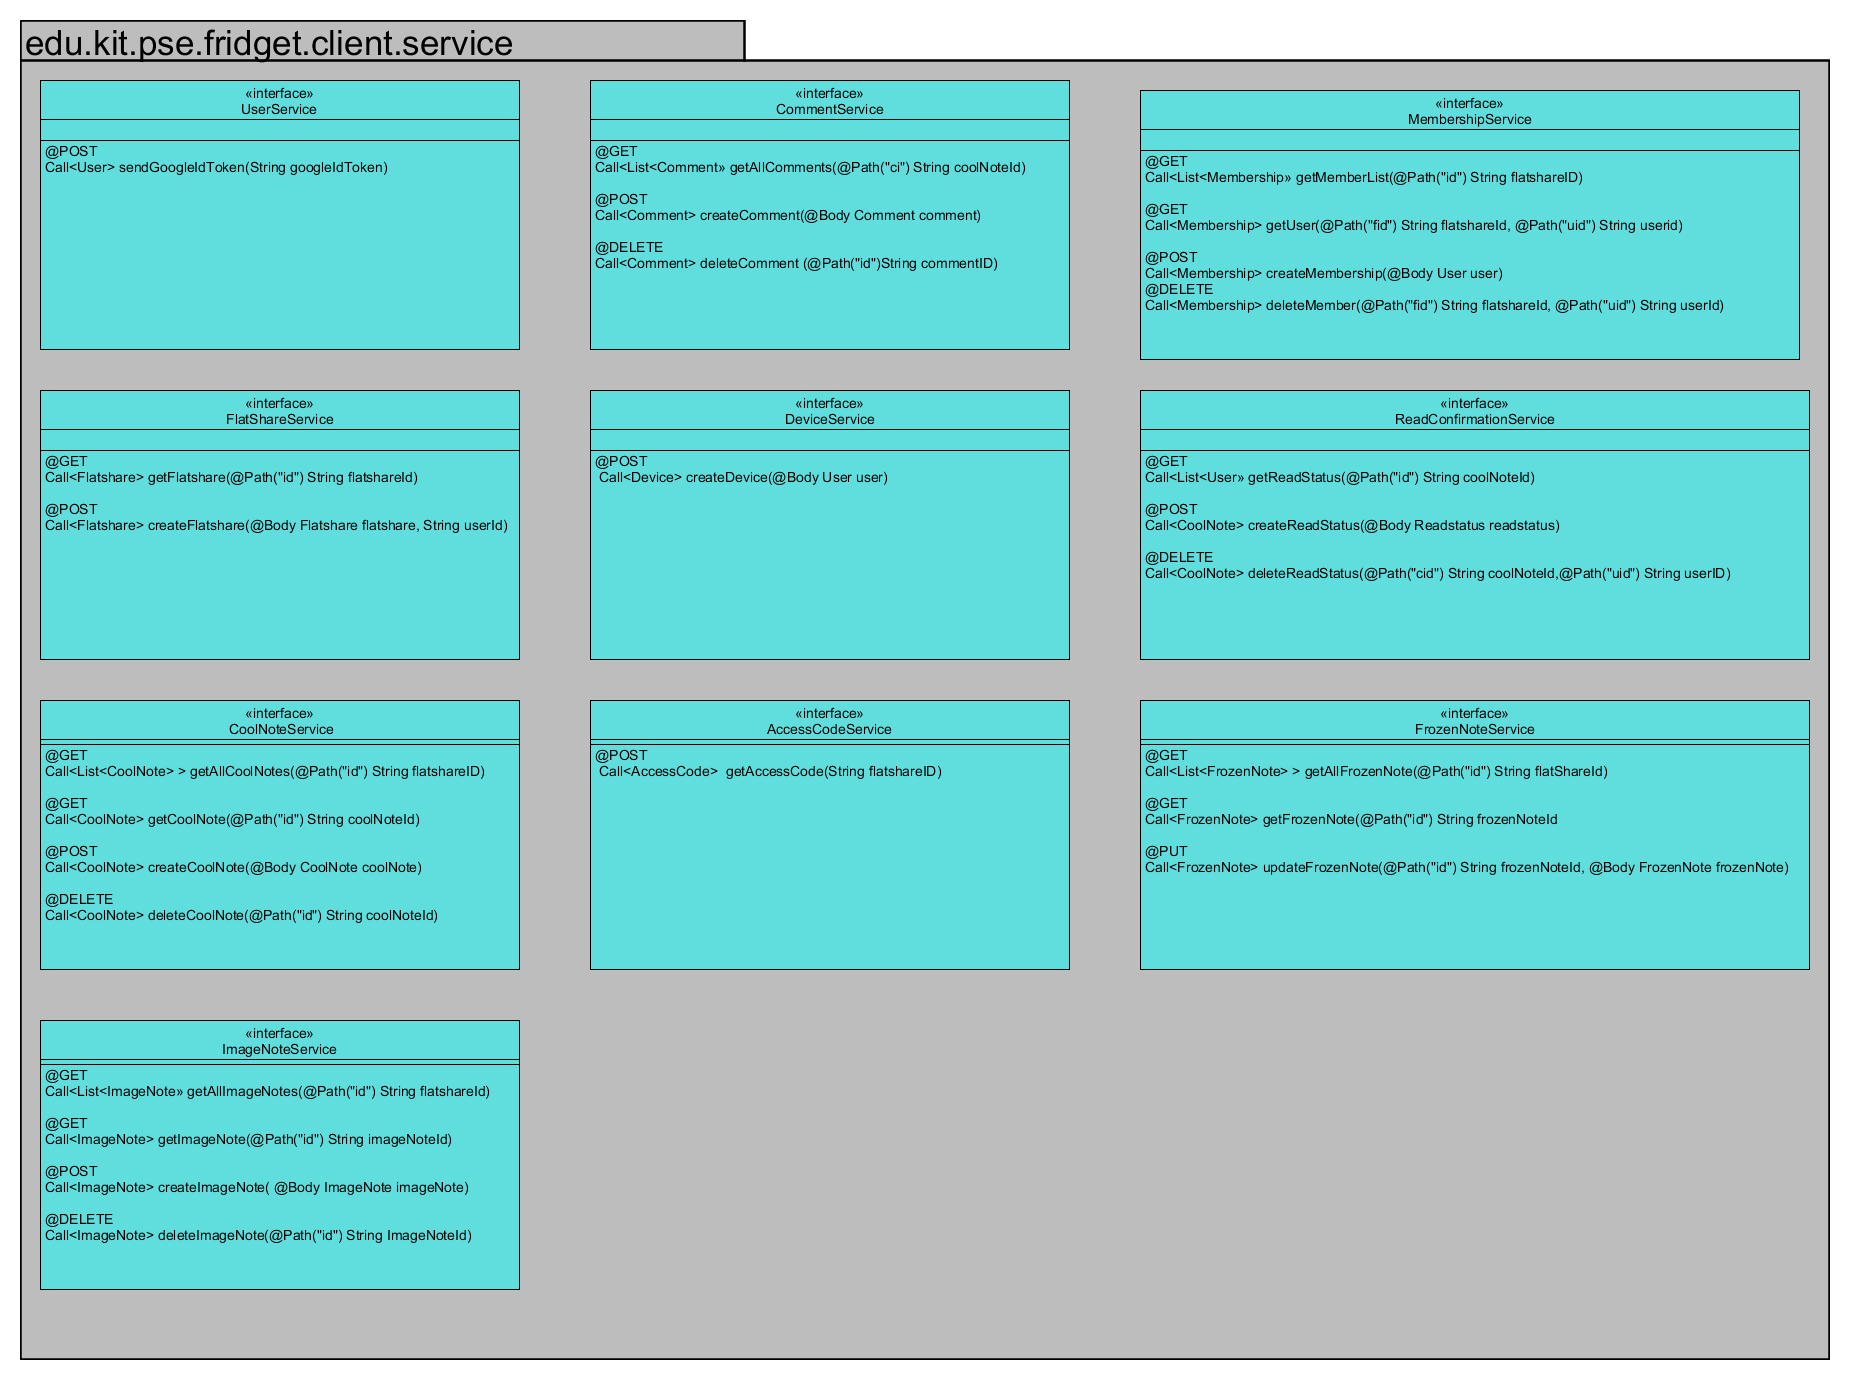
\includegraphics[scale = .26]{service.png}
	       \caption{Klassen des Services}
	      \end{figure}	
	\subsubsection{\texttt{public interface UserService}}
\textit{Dieses Interface dient dazu, es dem Nutzer zu ermöglichen, seinen bestehenden Google-Account zum Login zu verwenden. Dabei sendet der Client beim Login einen Token, welchen er vom Google-Server erhält. Dort wird der Token an den Server gesendet, dadurch erhält er die Google-Client-ID. Diese wird dauerhaft gespeichert.}\\

	\textbf{Methoden} \\
		\begin{itemize}
		\item{@GET\\ Call<User> getGoogleIdToken(String loginData)}

		\textit{Diese Methode ruft den GoogleToken vom Goolge API Server ab}

		\textbf{Parameter} \\
	loginData - Logindaten des Users

		\textbf{Rückgabewert} \\
	GoogleToken

      \item{@POST\\ Call<User> sendGoogleIdToken(String googleIdToken)}

		\textit{Diese Methode sendet den GoogleIdToken an den Server}

		\textbf{Parameter} \\
		googleIdToken - zu sendender GoogleToken

		\textbf{Rückgabewert} \\
	

	 \end{itemize}

	\subsubsection{\texttt{public interface AccessCodeService}}
\textit{Dieses Interface ist für die Synchronisation des Accesscodes mit dem Server zuständig }\\
\\
	\textbf{Methoden} \\
		\begin{itemize}
		\item{Call<AccessCode> getAccessCode(String flatShareID)}

		\textit{Diese Methode fordert den Accesscode einer Flatshare an}

		\textbf{Parameter} \\
	flatshareId - übergebende ID der Flatshare

		\textbf{Rückgabewert} \\
	Accesscode der Flatshare


	 \end{itemize}

		\subsubsection{\texttt{public interface CommentService }}
\textit{Dieses Interface ist für die Synchronisation der Comments mit dem Server zuständig}\\
\\
	\textbf{Methoden} \\
		\begin{itemize}
		\item{@GET("comments?cool-note=\{cid\}")\\ Call<List<Comment>> getAllComments(@Path(\grqq cid\grqq)String coolNoteId)}

		\textit{Diese Methode ruft alle Kommentare einer Cool Note ab}

		\textbf{Parameter} \\
	 coolNoteId - die Id der Cool Note 

		\textbf{Rückgabewert} \\
	Alle Comments der zur CoolNoteId gehörenden Cool Note


      \item{@POST("/comments")
\\ Call<Comment> createComment(@Body Comment comment)}

		\textit{Diese Methode schickt einen Comment an den Server }

		\textbf{Parameter} \\
		 comment - speichert einen Comment

		\textbf{Rückgabewert} \\
	Ein Comment

	 \item{@DELETE("/comments/{id}")\\ Call<Comment> deleteComment (@Path(\grqq id\grqq)String commentID)}

		\textit{Diese Methode löscht einen Comment }

		\textbf{Parameter} \\
		 commentID - ID des zu löschenden Comments 



	 \end{itemize}


	\subsubsection{\texttt{public interface CoolNoteService }}
\textit{Dieses Interface ist für die Synchronisation der Cool Notes mit dem Server zuständig}\\
\\
	\textbf{Methoden} \\
		\begin{itemize}
		\item{@GET("/cool-notes?flatshare={id}")\\ Call<List<CoolNote>> getAllCoolNotes(@Path(\grqq id\grqq) String flatshareID)} 

		\textit{Diese Methode ruft alle Cool Notes einer Flatshare ab}

		\textbf{Parameter} \\
	flatshareId - Die Flatshare der abzurufenden Cool Notes

		\textbf{Rückgabewert} \\
	Alle Cool Notes

      \item{@GET("/cool-notes/{id}")\\ Call<CoolNote> getCoolNote(@Path(\grqq id\grqq) String coolNoteId)}

		\textit{Diese Methode ruft den Inhalt einer Cool Note ab }

		\textbf{Parameter} \\
		coolNoteId - Die Id der Cool Note 

		\textbf{Rückgabewert} \\
	Inhalt der zu der CoolNoteId gehörenden Cool Note

      \item{@POST("/cool-notes")\\ Call<CoolNote> createCoolNote(@Body CoolNote coolNote)}

		\textit{Diese Methode schickt eine neue Cool Note an den Server }

		\textbf{Parameter} \\
		coolNoteI - Die Cool Note 

		\textbf{Rückgabewert} \\
	Cool Note


      \item{@DELETE("/cool-notes/{id}")\\ Call<CoolNote> deleteCoolNote(@Path(\grqq id\grqq) String coolNoteId)}

		\textit{Diese Methode löscht eine Cool Note }

		\textbf{Parameter} \\
		coolNoteId - Die Id der Cool Note 


	 \end{itemize}


	\subsubsection{\texttt{public interface FlatShareService }}
\textit{Dieses Interface verwaltet die Synchronisation der Flatshare mit dem Server}\\
\\
	\textbf{Methoden} \\
		\begin{itemize}
		\item{@POST ("/flatshares") \\
Call<Flatshare> createFlatshare(@Body Flatshare flatshare, String userId)
}

		\textit{Diese Methode erstellt eine neue Flatshare auf dem Server
}

		\textbf{Parameter} \\
	flatshare - Name der zu erstellenden Flatshare
	userID - ID des Users, der die Flatshare erstellt

		\textbf{Rückgabewert} \\
	Flatshare

      \item{@GET("/flatshares/{id}")\\ Call<Flatshare> getFlatshare(@Path(\grqq id\grqq) 					String flatshareId)}

		\textit{Diese Methode ruft die Flatshare-Daten vom Server ab}

		\textbf{Parameter} \\
		flatshareId - die ID der aufgerufenen Flatshare 

		\textbf{Rückgabewert} \\
	Flatshare


	 \end{itemize}



	\subsubsection{\texttt{public interface FrozenNoteService }}
\textit{Dieses Interface ist für die Synchronisation der Frozen Notes mit dem Server zuständig}\\
\\
	\textbf{Methoden} \\
		\begin{itemize}
		\item{@GET("/frozen-notes?flatshare={id}")\\
Call<List<FrozenNote>> getAllFrozenNote(@Path(\grqq id\grqq) String flatShareId)}

		\textit{Diese Methode ruft die Frozen Notes vom Server ab}

		\textbf{Parameter} \\
	flatshareId -  die ID der aufgerufenen Flatshare  

		\textbf{Rückgabewert} \\
	Frozen Note

      \item{@GET("/frozen-notes/{id}")\\ Call<FrozenNote> getFrozenNote(@Path(\grqq id\grqq) String frozenNoteId)}

		\textit{Diese Methode ruft den Inhalt einer Frozen Note ab }

		\textbf{Parameter} \\
		frozenNoteId - die ID der aufgerufenen Frozen Note  

		\textbf{Rückgabewert} \\
	FrozenNote

	 \item{@PUT("/frozen-notes/{id}")\\ Call<FrozenNote> updateFrozenNote(@Path(\grqq id\grqq) String frozenNoteId, @Body FrozenNote frozenNote)}

		\textit{Diese Methode speichert Änderungen in einer Frozen Note}

		\textbf{Parameter} \\
		frozenNoteId - die ID der aufgerufenen Frozen Note  
		frozenNote - die geänderte Frozen Note
		\textbf{Rückgabewert} \\
	FrozenNote

	 \end{itemize}


	\subsubsection{\texttt{public interface ImageNoteService }}
\textit{Dieses Interface dient zur Synchronisation der Image-Cool-Notes mit dem Server}\\
\\
	\textbf{Methoden} \\
		\begin{itemize}
		\item{@GET("/image-notes?flatshare={id}")\\
Call<List<ImageNote>> getAllImageNotes(@Path(\grqq id\grqq) String flatshareId)}

		\textit{Diese Methode ruft die Image-Cool-Notes vom Server ab}

		\textbf{Parameter} \\
	flatshareId - die ID der aufgerufenen Flatshare   

		\textbf{Rückgabewert} \\
	ImageCoolNote

      \item{@GET("/image-notes/{id}")\\ Call<ImageNote> getImageNote(@Path("\grqq id\grqq") String imageNoteId)}

		\textit{Diese Methode ruft eine Image-Cool-Note ab }

		\textbf{Parameter} \\
		 imageNoteId - die ID der aufgerufenen Image-Cool-Note  

		\textbf{Rückgabewert} \\
	Image-Cool-Note

	\item{@POST("/image-notes")\\ Call<ImageNote> createImageNote( @Body ImageNote imageNote)}

		\textit{Diese Methode schickt ein Image-Cool-Note an den Server}

		\textbf{Parameter} \\
		 imageNote - eine Image-Cool-Note  

		\textbf{Rückgabewert} \\
	Image-Cool-Note

	     \item{@DELETE("/image-notes/{id}")\\Call<ImageNote> deleteImageNote(@Path("\grqq id\grqq") String ImageNoteId)}

		\textit{Diese Methode löscht eine Image-Cool-Note}

		\textbf{Parameter} \\
		 imageNoteId - Die ID der zu löschenden Image-Cool-Note  

	 \end{itemize}


	\subsubsection{\texttt{public interface MembershipService }}
\textit{Dieses Interface verwaltet die Synchronisation der Members mit dem Server}\\
\\
	\textbf{Methoden} \\
		\begin{itemize}
		\item{@GET("/memberships/users?flatshare={id}") \\ Call<List<Membership>> getMemberList(@Path("id") String flatshareID)}

		\textit{Diese Methode ruft die Mitglieder einer Flatshare ab}

		\textbf{Parameter} \\
	flatshareId - die ID der aufgerufenen Flatshare  

		\textbf{Rückgabewert} \\
	MemberList

      \item{@GET("memberships?flatshare={fid}\&user ={uid}")\\Call<Membership> getUser(@Path("fid") String flatshareId, @Path(\grqq uid\grqq) String userid)}

		\textit{Diese Methode ruft die Daten eines Members ab}        	
		\textbf{Parameter} \\
		flatshareId - die ID der aufgerufenen Flatshare 
		userId - die ID des aufgerufenen Users

		\textbf{Rückgabewert} \\
      Daten eines Members


      \item{@POST("/memberships")\\ Call<Membership> createMembership(@Body User user)}

		\textit{Diese Methode fügt einen neuen Member in eine Flatshare ein}        	
		\textbf{Parameter} \\
		user - Der User, der zu der Flatshare hinzugefügt wird 

	      \item{@DELETE("/memberships?flatshare={fid}\&user={uid}")\\Call<Membership> deleteMember(@Path("fid") String flatshareId, @Path("uid") String userId)}

		\textit{Diese Methode löscht einen Member}        	
		\textbf{Parameter} \\
		flatshareId - die ID der aufgerufenen Flatshare 
		userId - die ID des aufgerufenen Users


	 \end{itemize}

	\subsubsection{\texttt{public interface ReadConfirmationService }}
\textit{Dieses Interface synchronisiert den Gelesen-Status mit dem Server}\\
\\
	\textbf{Methoden} \\

    \begin{itemize}
		\item{@GET("/read-confirmations/users?cool-note={id}") \\ Call<List<User>> getReadStatus(@Path(\grqq id\grqq) String coolNoteId)}

		\textit{Diese Methode ruft den Gelesen-Status vom Server ab}

		\textbf{Parameter} \\
	 coolNoteId - Die ID der betreffenden Cool Note

		\textbf{Rückgabewert} \\
	Read-Status

	\item{@POST("/read-confirmations") \\ Call<CoolNote> createReadStatus(@Body Readstatus readstatus) } \todo{Mins Klasse übernehmen}

		\textit{Diese Methode setzt die Checkbox auf markiert}

		\textbf{Parameter} \\
	 readstatus - zeigt den Gelesen-Status einer Cool Note an

		\textbf{Rückgabewert} \\
	ReadStatus



	\item{@DELETE("/read-confirmations?cool-note={cid}\&user={uid}")}
\\Call<CoolNote> deleteReadStatus(@Path("cid") String coolNoteId,
			     @Path(\grqq uid\grqq) String userID);

		\textit{Diese Methode setzt die Checkbox auf unmarkiert}

		\textbf{Parameter} \\
	coolNoteID - die ID der aufgerufenen Cool Note
	userID - die ID des aufgerufenen Users

	
	 \end{itemize}


	\subsubsection{\texttt{public interface DeviceService }}
\textit{Dieses Interface synchronisiert die Device-Daten mit dem Server}\\
\\
	\textbf{Methoden} \\
		\begin{itemize}
		\item{@POST("/devices") \\ Call<Device> createDevice(@Body User user)}

		\textit{Diese Methode fügt ein Device zu einer Flatshare hinzu}

		\textbf{Parameter} \\
	 user - der zu dem Device gehörende User 

		\textbf{Rückgabewert} \\


	 \end{itemize}
	\clearpage
	\section{RESTful API}
	%\documentclass[a4paper]{scrreprt}

%\usepackage[german]{babel}
%\usepackage[utf8]{inputenc}
%\usepackage[T1]{fontenc}
%\usepackage{ae}
%\usepackage[bookmarks,bookmarksnumbered]{hyperref}
%\usepackage{tocbasic}
%\usepackage{longtable}

%\begin{document}
    \subsection{HTTP-Protokoll}
    Folgende REST Endpoints verwenden wir für die Kommunikation zwischen Client und Server:
	\begin{flushleft}
		\begin{longtable}{|p{.12\textwidth}|p{.48\textwidth}|p{.4\textwidth}|}
		\hline
		\textbf{HTTP Methode} & \textbf{Endpoint} & \textbf{Beschreibung} \\
		\hline
		\multicolumn{3}{|l|} {FlatshareController} \\
		\hline
		GET & /flatshares/\{id\} & WG beitreten \\
		POST & /flatshares & WG erstellen \\ 
		\hline
		\multicolumn{3}{|l|}{AccessCodeController} \\
		\hline
		POST & /access-codes & Zugangscode anfordern \\ \hline
		\multicolumn{3}{|l|}{User} \\
		\hline
		POST & /users & Anmelden \\
		\hline
		\multicolumn{3}{|l|}{Device} \\
		\hline
		POST & /devices & App-Instanz-ID speichern \\
		\hline
		\multicolumn{3}{|l|}{MembershipController} \\
		\hline
		GET & /memberships/users?flatshare=\{id\} & Mitglieder ansehen \\
		GET & /memberships?flatshare=\{fid\}\&user=\{uid\} & Zugeteilte Magnetfarbe anfordern \\
		POST & /memberships & WG beitreten (mit Zugangscode) \\
		DELETE & /memberships?flatshare=\{fid\}\&user=\{uid\} & WG verlassen \\
		\hline
		\multicolumn{3}{|l|}{CoolNoteController} \\
		\hline
		GET & /cool-notes?flatshare=\{id\} & Cool Notes aktualisieren \\
		GET & /cool-notes/\{id\} & Großansicht einer Cool Note ansehen \\
		POST & /cool-notes & Cool Note erstellen \\
		DELETE & /cool-notes/\{id\} & Cool Note löschen \\
		\hline
		\multicolumn{3}{|l|}{FrozenNoteController} \\
		\hline
		GET & /frozen-notes?flatshare=\{id\} & Frozen Notes aktualisieren \\
		GET & /frozen-notes/\{id\} & Großansicht einer Frozen Note ansehen \\
		PUT & /frozen-notes/\{id\} & Frozen Note bearbeiten \\
		\hline
		\multicolumn{3}{|l|}{ImageNoteController} \\
		\hline
		GET & /image-notes?flatshare=\{id\} & Image Cool Notes aktualisieren \\
		GET & /image-notes/\{id\} & Großansicht einer Image Cool Note ansehen \\
		POST & /image-notes & Image Cool Note erstellen \\
		DELETE & /image-notes/\{id\} & Image Cool Note löschen \\
		\hline	
		\multicolumn{3}{|l|}{ReadConfirmationController} \\
		\hline
		GET & /read-confirmations/users?cool-note=\{id\} & Leser einer Cool Note ansehen \\
		POST & /read-confirmations & ``I have seen this''-Checkbox markieren \\
		DELETE & /read-confirmations?cool-note=\{cid\}\&user=\{uid\} & ``I have seen this''-Checkbox unmarkieren \\
		\hline
		\multicolumn{3}{|l|}{CommentController} \\
		\hline
		GET & /comments?cool-note=\{cid\} & Kommentare einer Cool Note ansehen \\
		POST & /comments & Kommentar schreiben \\
		DELETE & /comments/\{id\} & Kommentar löschen \\
		\hline
		\end{longtable}
	\end{flushleft}
	
	\subsection{HTTP-Statuscodes}
	Folgende Statuscodes liefern wir intern bei der HTTP-Antwort auf jede HTTP-Anfrage:
	\begin{flushleft}
		\begin{tabular}{|p{.15\textwidth}|p{.3\textwidth}|p{.55\textwidth}|}
		\hline
		\textbf{Code} & \textbf{Nachricht} & \textbf{Bedeutung} \\
		\hline
		\multicolumn{3}{|l|}{Erfolgreiche Operation} \\
		\hline
		200 & OK & Die Anfrage wurde erfolgreich bearbeitet und das Ergebnis der Anfrage wird in der Antwort übertragen. \\
		201 & Created & Die Anfrage wurde erfolgreich bearbeitet. Die angeforderte Ressource wurde vor dem Senden der Antwort erstellt. \\
		204 & No Content & Die Anfrage wurde erfolgreich durchgeführt, die Antwort enthält jedoch bewusst keine Daten. \\
		\hline
		\multicolumn{3}{|l|}{Client-Fehler} \\
		\hline
		400 & Bad Request & Die Anfrage-Nachricht war fehlerhaft aufgebaut. \\
		401 & Unauthorized & Die Anfrage kann nicht ohne gültige Authentifizierung durchgeführt werden. \\
		403 & Forbidden & Die Anfrage wurde mangels Berechtigung des Clients nicht durchgeführt, bspw. weil der authentifizierte Benutzer nicht berechtigt ist. \\
		404 & Not Found & Die angeforderte Ressource wurde nicht gefunden. \\
		422 & Unprocessable Entity & Die Verarbeitung der Anfrage wird z.B. wegen semantischer Fehler abgelehnt. \\
		\hline
		\multicolumn{3}{|l|}{Server-Fehler} \\
		\hline
		500 & Internal Server Error & Dies ist ein „Sammel-Statuscode“ für unerwartete Serverfehler. \\
		\hline	
		\end{tabular}
	\end{flushleft}
%\end{document}
	\clearpage
	\section{Klassen des Servers}
		\subsection{Klassendiagramm}
		\begin{figure}[H]
	       \centering
	       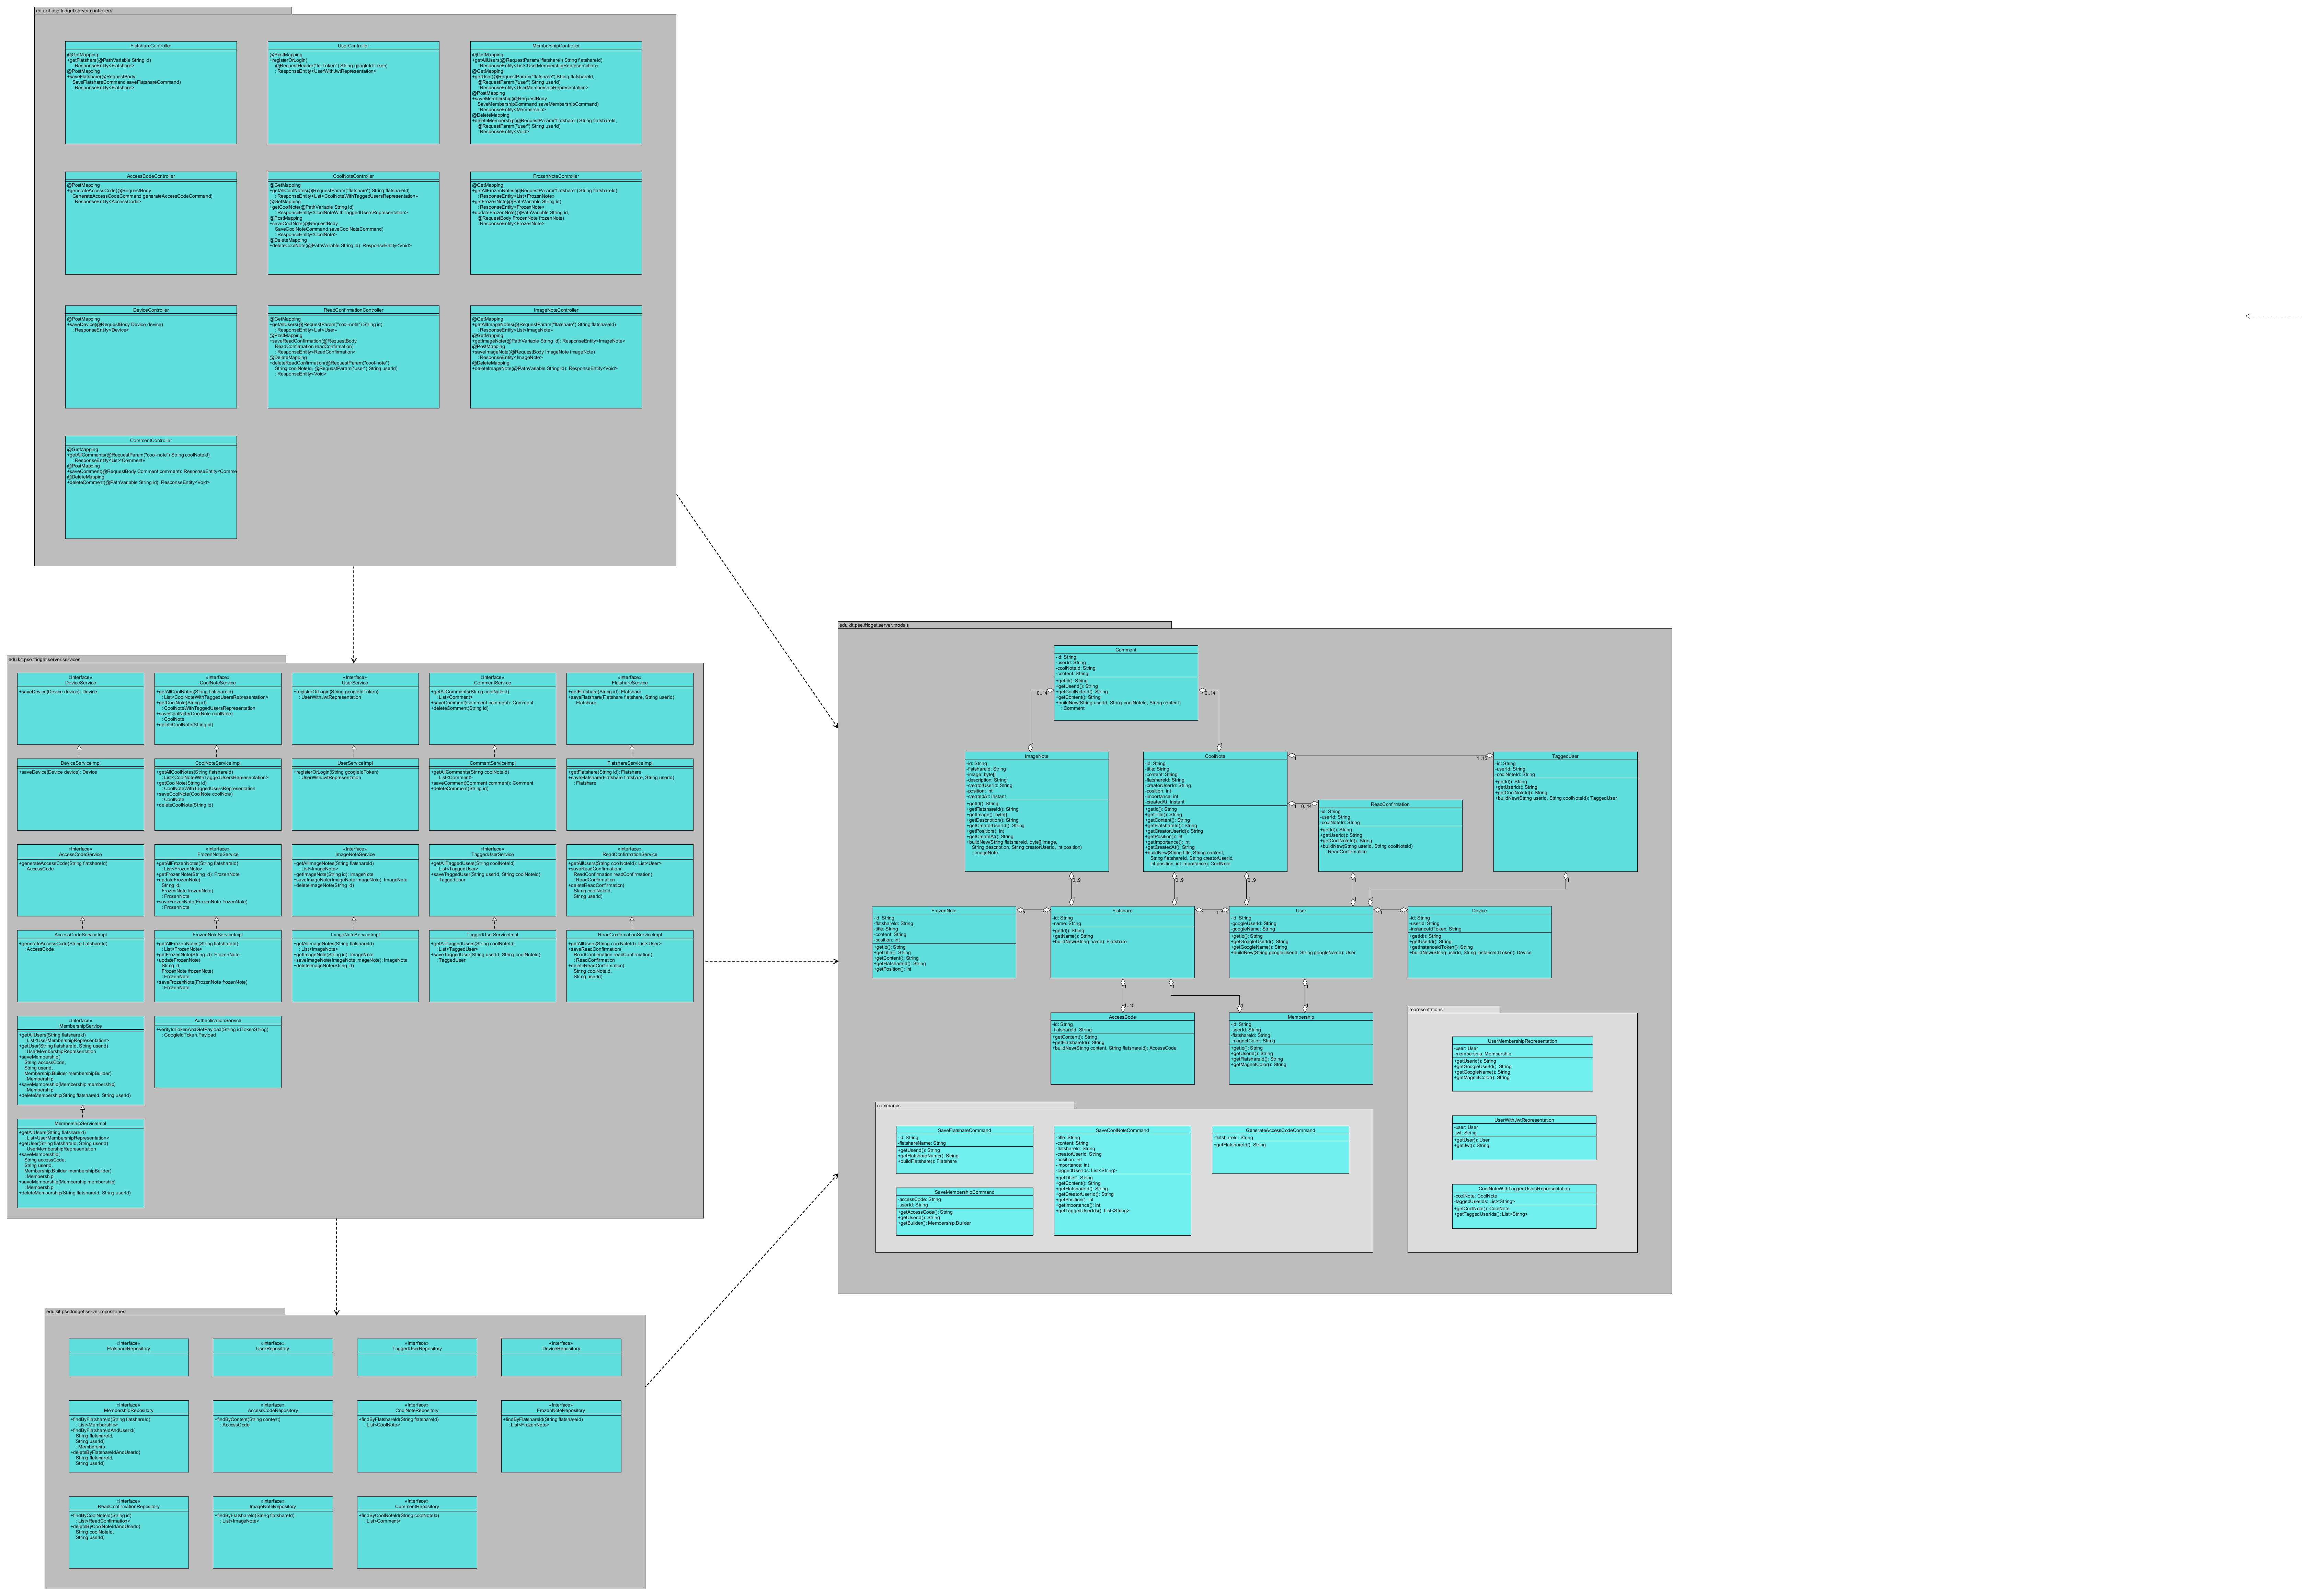
\includegraphics[scale = .05]{server-packages.png}
	       \caption{Klassen des Servers}
	      \end{figure}

	%\documentclass[a4paper]{scrreprt}

%\usepackage[german]{babel}
%\usepackage[utf8]{inputenc}
%\usepackage[T1]{fontenc}
%\usepackage{ae}
%\usepackage{tocbasic}

%\begin{document}
    \section{Package edu.kit.pse.fridget.server.controllers}
    \subsection{\texttt{Class AccessCodeController}}
    \textbf{Beschreibung} \\
    \textit{Controller für Zugangscode}
    \subsubsection{Konstruktor}
    \texttt{public AccessCodeController(AccessCodeService service)}
    \subsubsection{Methoden}
    \begin{itemize}
    	\item{\texttt{public ResponseEntity<AccessCode> generateAccessCode(GenerateAccessCodeCommand generateAccessCodeCommand)}}
    	
    	\textit{Generiert einen Zugangscode für eine WG.}
    	
    	\textbf{Parameter} \\
    	generateAccessCodeCommand WG-ID
    	
    	\textbf{Rückgabewert} \\
    	Generierter Zugangscode als ResponseEntity
    \end{itemize}
    \subsection{\texttt{Class CommentController}}
    \textbf{Beschreibung} \\
    \textit{Controller für Kommentar}
    \subsubsection{Konstruktor}
    \texttt{public CommentController(CommentService service)}
    \subsubsection{Methoden}
    \begin{itemize}
    	\item{\texttt{public ResponseEntity<List<Comment$>>$ getAllComments(String coolNoteId)}}
    	
    	\textit{Findet alle Kommentare zu einer Cool Note.}
    	
    	\textbf{Parameter} \\
    	coolNoteId CoolNote-ID
    	
    	\textbf{Rückgabewert} \\
    	Liste von gefundenen Kommentaren als ResponseEntity        \item{\texttt{public ResponseEntity<Comment> saveComment(Comment comment)}}
    	
    	\textit{Speichert einen Kommentar.}
    	
    	\textbf{Parameter} \\
    	comment Kommentar zum speichern
    	
    	\textbf{Rückgabewert} \\
    	Gespeicherter Kommentar als ResponseEntity        \item{\texttt{public ResponseEntity<Void> deleteComment(String id)}}
    	
    	\textit{Löscht einen Kommentar.}
    	
    	\textbf{Parameter} \\
    	id Kommentar-ID
    	
    	\textbf{Rückgabewert} \\
    	Leere ResponseEntity
    \end{itemize}
    \subsection{\texttt{Class CoolNoteController}}
    \textbf{Beschreibung} \\
    \textit{Controller für Cool Note}
    \subsubsection{Konstruktor}
    \texttt{public CoolNoteController(CoolNoteService coolNoteService, TaggedUserService taggedUserService)}
    \subsubsection{Methoden}
    \begin{itemize}
    	\item{\texttt{public ResponseEntity<List<CoolNoteWithTaggedUsersRepresentation$>>$ getAllCoolNotes(String flatshareId)}}
    	
    	\textit{Findet alle Cool Notes mit getaggten Benutzern in einer WG.}
    	
    	\textbf{Parameter} \\
    	flatshareId WG-ID
    	
    	\textbf{Rückgabewert} \\
    	Liste von gefundenen CoolNote mit ID von getaggten Benutzern als ResponseEntity        \item{\texttt{public ResponseEntity<CoolNoteWithTaggedUsersRepresentation> getCoolNote(String id)}}
    	
    	\textit{Findet eine Cool Note mit getaggten Benutzern.}
    	
    	\textbf{Parameter} \\
    	id CoolNote-ID
    	
    	\textbf{Rückgabewert} \\
    	Gefundene CoolNote mit ID von getaggten Benutzern als ResponseEntity        \item{\texttt{public ResponseEntity<CoolNote> saveCoolNote(SaveCoolNoteCommand saveCoolNoteCommand)}}
    	
    	\textit{Speichert eine Cool Note and die getaggten Benutzer.}
    	
    	\textbf{Parameter} \\
    	saveCoolNoteCommand CoolNote mit ID von getaggten Benutzern zum speichern
    	
    	\textbf{Rückgabewert} \\
    	Gespeicherte CoolNote als ResponseEntity        \item{\texttt{public ResponseEntity<Void> deleteCoolNote(String id)}}
    	
    	\textit{Löscht eine Cool Note.}
    	
    	\textbf{Parameter} \\
    	id CoolNote-ID
    	
    	\textbf{Rückgabewert} \\
    	Leere ResponseEntity
    \end{itemize}
    \subsection{\texttt{Class DeviceController}}
    \textbf{Beschreibung} \\
    \textit{Controller für Gerät}
    \subsubsection{Konstruktor}
    \texttt{public DeviceController(DeviceService service)}
    \subsubsection{Methoden}
    \begin{itemize}
    	\item{\texttt{public ResponseEntity<Device> saveDevice(Device device)}}
    	
    	\textit{Speichert ein neues Gerät.}
    	
    	\textbf{Parameter} \\
    	device Gerät zum speichern
    	
    	\textbf{Rückgabewert} \\
    	Gespeichertes Gerät als ResponseEntity
    \end{itemize}
    \subsection{\texttt{Class FlatshareController}}
    \textbf{Beschreibung} \\
    \textit{Controller für WG}
    \subsubsection{Konstruktor}
    \texttt{public FlatshareController(FlatshareService service)}
    \subsubsection{Methoden}
    \begin{itemize}
    	\item{\texttt{public ResponseEntity<Flatshare> getFlatshare(String id)}}
    	
    	\textit{Findet eine WG.}
    	
    	\textbf{Parameter} \\
    	id WG-ID
    	
    	\textbf{Rückgabewert} \\
    	Gefundene WG als ResponseEntity        \item{\texttt{public ResponseEntity<Flatshare> saveFlatshare(SaveFlatshareCommand saveFlatshareCommand)}}
    	
    	\textit{Speichert eine WG.}
    	
    	\textbf{Parameter} \\
    	saveFlatshareCommand WG zum speichern
    	
    	\textbf{Rückgabewert} \\
    	Gespeicherte WG als ResponseEntity
    \end{itemize}
    \subsection{\texttt{Class FrozenNoteController}}
    \textbf{Beschreibung} \\
    \textit{Controller für Frozen Note}
    \subsubsection{Konstruktor}
    \texttt{public FrozenNoteController(FrozenNoteService service)}
    \subsubsection{Methoden}
    \begin{itemize}
    	\item{\texttt{public ResponseEntity<List<FrozenNote$>>$ getAllFrozenNotes(String flatshareId)}}
    	
    	\textit{Findet alle Frozen Notes in einer WG.}
    	
    	\textbf{Parameter} \\
    	flatshareId WG-ID
    	
    	\textbf{Rückgabewert} \\
    	Liste von gefundenen FrozenNote als ResponseEntity        \item{\texttt{public ResponseEntity<FrozenNote> getFrozenNote(String id)}}
    	
    	\textit{Findet eine Frozen Note.}
    	
    	\textbf{Parameter} \\
    	id FrozenNote-ID
    	
    	\textbf{Rückgabewert} \\
    	Gefundene FrozenNote als ResponseEntity        \item{\texttt{public ResponseEntity<FrozenNote> updateFrozenNote(String id, FrozenNote frozenNote)}}
    	
    	\textit{Updatet eine Frozen Note.}
    	
    	\textbf{Parameter} \\
    	id FrozenNote-ID
    	frozenNote FrozenNote zum updaten
    	
    	\textbf{Rückgabewert} \\
    	Geupdatete FrozenNote als ResponseEntity
    \end{itemize}
    \subsection{\texttt{Class ImageNoteController}}
    \textbf{Beschreibung} \\
    \textit{Controller für Image Cool Note}
    \subsubsection{Konstruktor}
    \texttt{public ImageNoteController(ImageNoteService service)}
    \subsubsection{Methoden}
    \begin{itemize}
    	\item{\texttt{public ResponseEntity<List<ImageNote$>>$ getAllImageNotes(String flatshareId)}}
    	
    	\textit{Findet alle Image Cool Notes in einer WG.}
    	
    	\textbf{Parameter} \\
    	flatshareId WG-ID
    	
    	\textbf{Rückgabewert} \\
    	Liste von gefundenen ImageNote als ResponseEntity        \item{\texttt{public ResponseEntity<ImageNote> getImageNote(String id)}}
    	
    	\textit{Findet eine Image Cool Note.}
    	
    	\textbf{Parameter} \\
    	id ImageNote-ID
    	
    	\textbf{Rückgabewert} \\
    	Gefundene ImageNote als ResponseEntity        \item{\texttt{public ResponseEntity<ImageNote> saveImageNote(ImageNote imageNote)}}
    	
    	\textit{Speichert eine Image Cool Note.}
    	
    	\textbf{Parameter} \\
    	imageNote ImageNote zum speichern
    	
    	\textbf{Rückgabewert} \\
    	Gespeicherte ImageNote als ResponseEntity        \item{\texttt{public ResponseEntity<Void> deleteImageNote(String id)}}
    	
    	\textit{Löscht eine Image Cool Note.}
    	
    	\textbf{Parameter} \\
    	id ImageNote-ID
    	
    	\textbf{Rückgabewert} \\
    	Leere ResponseEntity
    \end{itemize}
    \subsection{\texttt{Class MembershipController}}
    \textbf{Beschreibung} \\
    \textit{Controller für Mitgliedschaft}
    \subsubsection{Konstruktor}
    \texttt{public MembershipController(MembershipService service)}
    \subsubsection{Methoden}
    \begin{itemize}
    	\item{\texttt{public ResponseEntity<List<UserMembershipRepresentation$>>$ getAllUsers(String flatshareId)}}
    	
    	\textit{Findet alle Mitglieder in einer WG.}
    	
    	\textbf{Parameter} \\
    	flatshareId WG-ID
    	
    	\textbf{Rückgabewert} \\
    	Liste von gefundenen Benutzern mit Magenetfarben als ResponseEntity        \item{\texttt{public ResponseEntity<UserMembershipRepresentation> getUser(String flatshareId, String userId)}}
    	
    	\textit{Findet ein Mitglied in einer WG.}
    	
    	\textbf{Parameter} \\
    	flatshareId WG-ID
    	userId Benutzer-ID
    	
    	\textbf{Rückgabewert} \\
    	Gefundener Benutzer mit Magnetfarbe als ResponseEntity        \item{\texttt{public ResponseEntity<Membership> saveMembership(SaveMembershipCommand saveMembershipCommand)}}
    	
    	\textit{Speichert einen Benutzer in einer WG.}
    	
    	\textbf{Parameter} \\
    	saveMembershipCommand Benutzer-ID und Zugangscode
    	
    	\textbf{Rückgabewert} \\
    	Gespeicherte Mitgliedschaft als ResponseEntity        \item{\texttt{public ResponseEntity<Void> deleteMembership(String flatshareId, String userId)}}
    	
    	\textit{Löscht ein Mitglied von einer WG.}
    	
    	\textbf{Parameter} \\
    	flatshareId WG-ID
    	userId Benutzer-ID
    	
    	\textbf{Rückgabewert} \\
    	Leere ResponseEntity
    \end{itemize}
    \subsection{\texttt{Class ReadConfirmationController}}
    \textbf{Beschreibung} \\
    \textit{Controller für Lesebestätigung}
    \subsubsection{Konstruktor}
    \texttt{public ReadConfirmationController(ReadConfirmationService service)}
    \subsubsection{Methoden}
    \begin{itemize}
    	\item{\texttt{public ResponseEntity<List<User$>>$ getAllUsers(String id)}}
    	
    	\textit{Findet alle Leser einer Cool Note.}
    	
    	\textbf{Parameter} \\
    	id CoolNote-ID
    	
    	\textbf{Rückgabewert} \\
    	Liste von gefundenen Benutzern als ResponseEntity        \item{\texttt{public ResponseEntity<ReadConfirmation> saveReadConfirmation(ReadConfirmation readConfirmation)}}
    	
    	\textit{Speichert einen Benutzer als Leser einer Cool Note.}
    	
    	\textbf{Parameter} \\
    	readConfirmation Lesebestätigung zum speichern
    	
    	\textbf{Rückgabewert} \\
    	Gespeicherte Lesebestätigung als ResponseEntity        \item{\texttt{public ResponseEntity<Void> deleteReadConfirmation(String coolNoteId, String userId)}}
    	
    	\textit{Löscht einen Benutzer als Leser einer Cool Note.}
    	
    	\textbf{Parameter} \\
    	coolNoteId CoolNote-ID
    	userId Benutzer-ID
    	
    	\textbf{Rückgabewert} \\
    	Leere ResponseEntity
    \end{itemize}
    \subsection{\texttt{Class UserController}}
    \textbf{Beschreibung} \\
    \textit{Controller für Benutzer}
    \subsubsection{Konstruktor}
    \texttt{public UserController(UserService service)}
    \subsubsection{Methoden}
    \begin{itemize}
    	\item{\texttt{public ResponseEntity<UserWithJwtRepresentation> registerOrLogin(String googleIdToken)}}
    	
    	\textit{Authentifiziert einen Benutzer durch Google-ID-Token.}
    	
    	\textbf{Parameter} \\
    	googleIdToken Google-ID-Token
    	
    	\textbf{Rückgabewert} \\
    	Gespeicherter oder angemeldeter Benutzer mit JWT als ResponseEntity
    \end{itemize}
    \section{Package edu.kit.pse.fridget.server.models}
    \subsection{\texttt{Class AccessCode}}
    \textbf{Beschreibung} \\
    \textit{Model für Zugangscode}
    \subsubsection{Methoden}
    \begin{itemize}
    	\item{\texttt{public String getContent()}}
    	
    	\textit{Getter für Inhalt vom Zugangscode}
    	
    	
    	
    	\textbf{Rückgabewert} \\
    	Zugangscode-Inhalt        \item{\texttt{public String getFlatshareId()}}
    	
    	\textit{Getter für WG-ID}
    	
    	
    	
    	\textbf{Rückgabewert} \\
    	WG-ID        \item{\texttt{public AccessCode buildNew(String content, String flatshareId)}}
    	
    	\textit{Baut Zugangscode mit zufälliger UUID.}
    	
    	\textbf{Parameter} \\
    	content Inhalt vom Zugangscode
    	flatshareId ID von der WG, die mit dem Zugangscode beigetreten werden kann
    	
    	\textbf{Rückgabewert} \\
    	Gebauter Zugangscode mit zufälliger UUID
    \end{itemize}
    \subsection{\texttt{Class Comment}}
    \textbf{Beschreibung} \\
    \textit{Model für Kommentar}
    \subsubsection{Methoden}
    \begin{itemize}
    	\item{\texttt{public String getId()}}
    	
    	\textit{Getter für Kommentar-ID}
    	
    	
    	
    	\textbf{Rückgabewert} \\
    	Kommentar-ID        \item{\texttt{public String getUserId()}}
    	
    	\textit{Getter für ID von dem Benutzer, der den Kommentar geschrieben hat}
    	
    	
    	
    	\textbf{Rückgabewert} \\
    	Benutzer-ID        \item{\texttt{public String getCoolNoteId()}}
    	
    	\textit{Getter für ID von der Cool Note, der der Kommentar gehört zu}
    	
    	
    	
    	\textbf{Rückgabewert} \\
    	CoolNote-ID        \item{\texttt{public String getContent()}}
    	
    	\textit{Getter für Inhalt vom Kommentar}
    	
    	
    	
    	\textbf{Rückgabewert} \\
    	Kommentar-Inhalt        \item{\texttt{public Comment buildNew(String userId, String coolNoteId, String content)}}
    	
    	\textit{Baut Kommentar mit zufälliger UUID.}
    	
    	\textbf{Parameter} \\
    	userId ID von dem Benutzer, der den Kommentar geschrieben hat
    	coolNoteId ID von der Cool Note, der der Kommentar gehört zu
    	content Inhalt vom Kommentar
    	
    	\textbf{Rückgabewert} \\
    	Gebauter Kommentar mit zufälliger UUID
    \end{itemize}
    \subsection{\texttt{Class CoolNote}}
    \textbf{Beschreibung} \\
    \textit{Model für Cool Note}
    \subsubsection{Methoden}
    \begin{itemize}
    	\item{\texttt{public String getId()}}
    	
    	\textit{Getter für CoolNote-ID}
    	
    	
    	
    	\textbf{Rückgabewert} \\
    	CoolNote-ID        \item{\texttt{public String getTitle()}}
    	
    	\textit{Getter für Überschrift von der Cool Note}
    	
    	
    	
    	\textbf{Rückgabewert} \\
    	CoolNote-Überschrift        \item{\texttt{public String getContent()}}
    	
    	\textit{Getter für Inhalt von der Cool Note}
    	
    	
    	
    	\textbf{Rückgabewert} \\
    	CoolNote-Inhalt        \item{\texttt{public String getFlatshareId()}}
    	
    	\textit{Getter für ID von der WG, zu der diese Cool Note gehört}
    	
    	
    	
    	\textbf{Rückgabewert} \\
    	WG-ID        \item{\texttt{public String getCreatorUserId()}}
    	
    	\textit{Getter für ID vom Benutzer, der die Cool Note erstellt hat}
    	
    	
    	
    	\textbf{Rückgabewert} \\
    	Benutzer-ID        \item{\texttt{public int getPosition()}}
    	
    	\textit{Getter für Position der Cool Note auf der Pinnwand}
    	
    	
    	
    	\textbf{Rückgabewert} \\
    	Position der Cool Note        \item{\texttt{public int getImportance()}}
    	
    	\textit{Getter für Wichtigkeit der Cool Note}
    	
    	
    	
    	\textbf{Rückgabewert} \\
    	Wichtigkeit der Cool Note        \item{\texttt{public CoolNote buildNew(String title, String content, String flatshareId, String creatorUserId, int position, int importance)}}
    	
    	\textit{Baut Cool Note mit zufälliger UUID und aktuellem Datum.}
    	
    	\textbf{Parameter} \\
    	title Überschrift von der Cool Note
    	content Inhalt von der Cool Note
    	flatshareId ID von der WG, zu der diese Cool Note gehört
    	creatorUserId ID vom Benutzer, der die Cool Note erstellt hat
    	position Position der Cool Note auf der Pinnwand
    	importance Wichtigkeit der Cool Note
    	
    	\textbf{Rückgabewert} \\
    	Gebaute Cool Note mit zufälliger UUID und aktuellem Datum
    \end{itemize}
    \subsection{\texttt{Class Device}}
    \textbf{Beschreibung} \\
    \textit{Model für Gerät}
    \subsubsection{Methoden}
    \begin{itemize}
    	\item{\texttt{public String getId()}}
    	
    	\textit{Getter für ID vom Gerät}
    	
    	
    	
    	\textbf{Rückgabewert} \\
    	Gerät-ID        \item{\texttt{public String getUserId()}}
    	
    	\textit{Getter für ID vom Benutzer, der die App auf dem Gerät benutzt}
    	
    	
    	
    	\textbf{Rückgabewert} \\
    	Benutzer-ID        \item{\texttt{public String getInstanceIdToken()}}
    	
    	\textit{Getter für ID von der App-Instanz auf dem Gerät}
    	
    	
    	
    	\textbf{Rückgabewert} \\
    	Instanz-ID        \item{\texttt{public Device buildNew(String userId, String instanceIdToken)}}
    	
    	\textit{Baut Gerät mit zufälliger UUID.}
    	
    	\textbf{Parameter} \\
    	userId Benutzer-ID
    	instanceIdToken Instanz-ID-Token
    	
    	\textbf{Rückgabewert} \\
    	Gebautes Gerät mit zufälliger UUID
    \end{itemize}
    \subsection{\texttt{Class Flatshare}}
    \textbf{Beschreibung} \\
    \textit{Model für WG}
    \subsubsection{Methoden}
    \begin{itemize}
    	\item{\texttt{public String getId()}}
    	
    	\textit{Getter für WG-ID}
    	
    	
    	
    	\textbf{Rückgabewert} \\
    	WG-ID        \item{\texttt{public String getName()}}
    	
    	\textit{Getter für WG-Name}
    	
    	
    	
    	\textbf{Rückgabewert} \\
    	WG-Name        \item{\texttt{public Flatshare buildNew(String name)}}
    	
    	\textit{Baut WG mit zufälliger UUID.}
    	
    	\textbf{Parameter} \\
    	name Name von der WG
    	
    	\textbf{Rückgabewert} \\
    	Gebaute WG mit zufälliger UUID
    \end{itemize}
    \subsection{\texttt{Class FrozenNote}}
    \textbf{Beschreibung} \\
    \textit{Model für Frozen Note}
    \subsubsection{Methoden}
    \begin{itemize}
    	\item{\texttt{public String getId()}}
    	
    	\textit{Getter für FrozenNote-ID}
    	
    	
    	
    	\textbf{Rückgabewert} \\
    	FrozenNote-ID        \item{\texttt{public String getTitle()}}
    	
    	\textit{Getter für Überschrift von der Frozen Note}
    	
    	
    	
    	\textbf{Rückgabewert} \\
    	FronzenNote-Überschrift        \item{\texttt{public String getContent()}}
    	
    	\textit{Getter für Inhalt von der Frozen Note}
    	
    	
    	
    	\textbf{Rückgabewert} \\
    	FrozenNote-Inhalt        \item{\texttt{public String getFlatshareId()}}
    	
    	\textit{Getter für ID von der WG, zu der diese Frozen Note gehört}
    	
    	
    	
    	\textbf{Rückgabewert} \\
    	WG-ID
    \end{itemize}
    \subsection{\texttt{Class ImageNote}}
    \textbf{Beschreibung} \\
    \textit{Model für Image Cool Note}
    \subsubsection{Methoden}
    \begin{itemize}
    	\item{\texttt{public String getId()}}
    	
    	\textit{Getter für ImageNote-ID}
    	
    	
    	
    	\textbf{Rückgabewert} \\
    	ImageNote-ID        \item{\texttt{public String getFlatshareId()}}
    	
    	\textit{Getter für ID von der WG, zu der diese Image Cool Note gehört}
    	
    	
    	
    	\textbf{Rückgabewert} \\
    	WG-ID        \item{\texttt{public byte[] getImage()}}
    	
    	\textit{Getter für Bild in der Image Cool Note}
    	
    	
    	
    	\textbf{Rückgabewert} \\
    	Bild        \item{\texttt{public String getDescription()}}
    	
    	\textit{Getter für Beschreibung der Image Cool Note}
    	
    	
    	
    	\textbf{Rückgabewert} \\
    	Beschreibung der Image Cool Note        \item{\texttt{public String getCreatorUserId()}}
    	
    	\textit{Getter für ID vom Benutzer, der die Image Cool Note erstellt hat}
    	
    	
    	
    	\textbf{Rückgabewert} \\
    	Benutzer-ID        \item{\texttt{public int getPosition()}}
    	
    	\textit{Getter für Position der Image Cool Note auf der Pinnwand}
    	
    	
    	
    	\textbf{Rückgabewert} \\
    	Position der Image Cool Note        \item{\texttt{public ImageNote buildNew(String flatshareId, byte[] image, String description, String creatorUserId, int position)}}
    	
    	\textit{Baut Image Cool Note mit zufälliger UUID und aktuellem Datum.}
    	
    	\textbf{Parameter} \\
    	flatshareId ID von der WG, zu der diese Image Cool Note gehört
    	image Bild in der Image Cool Note
    	description Beschreibung der Image Cool Note
    	creatorUserId ID vom Benutzer, der die Image Cool Note erstellt hat
    	position Position der Image Cool Note auf der Pinnwand
    	
    	\textbf{Rückgabewert} \\
    	Gebaute Image Cool Note mit zufälliger UUID und aktuellem Datum
    \end{itemize}
    \subsection{\texttt{Class Membership}}
    \textbf{Beschreibung} \\
    \textit{Model für Mitgliedschaft}
    \subsubsection{Methoden}
    \begin{itemize}
    	\item{\texttt{public String getUserId()}}
    	
    	\textit{Getter für ID vom Mitglied}
    	
    	
    	
    	\textbf{Rückgabewert} \\
    	Benutzer-ID        \item{\texttt{public String getFlatshareId()}}
    	
    	\textit{Getter für WG-ID}
    	
    	
    	
    	\textbf{Rückgabewert} \\
    	WG-ID        \item{\texttt{public String getMagnetColor()}}
    	
    	\textit{Getter für Magnetfarbe, die dem Mitglied in der WG zugeteilt wird}
    	
    	
    	
    	\textbf{Rückgabewert} \\
    	Magenetfarbe
    \end{itemize}
    \subsection{\texttt{Class ReadConfirmation}}
    \textbf{Beschreibung} \\
    \textit{Model für Lesebestätigung}
    \subsubsection{Methoden}
    \begin{itemize}
    	\item{\texttt{public String getId()}}
    	
    	\textit{Getter für Lesebestätigung-ID}
    	
    	
    	
    	\textbf{Rückgabewert} \\
    	Lesebestätigung-ID        \item{\texttt{public String getUserId()}}
    	
    	\textit{Getter für ID vom Benutzer, der die Cool Note gelesen hat}
    	
    	
    	
    	\textbf{Rückgabewert} \\
    	Benutzer-ID        \item{\texttt{public String getCoolNoteId()}}
    	
    	\textit{Getter für ID vom Cool Note, die gelesen wurde}
    	
    	
    	
    	\textbf{Rückgabewert} \\
    	CoolNote-ID        \item{\texttt{public ReadConfirmation buildNew(String userId, String coolNoteId)}}
    	
    	\textit{Baut Lesebestätigung.}
    	
    	\textbf{Parameter} \\
    	userId ID vom Benutzer, der die Cool Note gelesen hat
    	coolNoteId ID vom Cool Note, die gelesen wurde
    	
    	\textbf{Rückgabewert} \\
    	Gebaute Lesebestätigung
    \end{itemize}
    \subsection{\texttt{Class TaggedUser}}
    \textbf{Beschreibung} \\
    \textit{Model für getaggte Mitglieder}
    \subsubsection{Methoden}
    \begin{itemize}
    	\item{\texttt{public String getId()}}
    	
    	\textit{Getter für ID vom getaggten Mitglied}
    	
    	
    	
    	\textbf{Rückgabewert} \\
    	ID vom getaggten Mitglied        \item{\texttt{public String getUserId()}}
    	
    	\textit{Getter für ID vom Benutzer, der getaggt wurde}
    	
    	
    	
    	\textbf{Rückgabewert} \\
    	Benutzer-ID        \item{\texttt{public String getCoolNoteId()}}
    	
    	\textit{Getter für ID von der Cool Note, in der der Benutzer getaggt wurde}
    	
    	
    	
    	\textbf{Rückgabewert} \\
    	CoolNote-ID        \item{\texttt{public TaggedUser buildNew(String userId, String coolNoteId)}}
    	
    	\textit{Baut getaggtes Mitglied.}
    	
    	\textbf{Parameter} \\
    	userId ID vom Benutzer, der getaggt wurde
    	coolNoteId ID von der Cool Note, in der der Benutzer getaggt wurde
    	
    	\textbf{Rückgabewert} \\
    	Gebautes getaggtes Mitglied
    \end{itemize}
    \subsection{\texttt{Class User}}
    \textbf{Beschreibung} \\
    \textit{Model für Benutzer}
    \subsubsection{Methoden}
    \begin{itemize}
    	\item{\texttt{public String getId()}}
    	
    	\textit{Getter für Benutzer-ID}
    	
    	
    	
    	\textbf{Rückgabewert} \\
    	Benutzer-ID        \item{\texttt{public String getGoogleUserId()}}
    	
    	\textit{Getter für Google-ID vom Benutzer}
    	
    	
    	
    	\textbf{Rückgabewert} \\
    	Google-ID        \item{\texttt{public String getGoogleName()}}
    	
    	\textit{Getter für Google-Name vom Benutzer}
    	
    	
    	
    	\textbf{Rückgabewert} \\
    	Google-Name        \item{\texttt{public User buildNew(String googleUserId, String googleName)}}
    	
    	\textit{Baut Benutzer mit zufälliger UUID.}
    	
    	\textbf{Parameter} \\
    	googleUserId Google-ID vom Benutzer
    	googleName Google-Name vom Benutzer
    	
    	\textbf{Rückgabewert} \\
    	Gebauter Benutzer mit zufälliger UUID
    \end{itemize}
    \section{Package edu.kit.pse.fridget.server.models.commands}
    \subsection{\texttt{Class GenerateAccessCodeCommand}}
    \textbf{Beschreibung} \\
    \textit{Model für das Generieren des Zugangscodes}
    \subsubsection{Konstruktor}
    \texttt{public GenerateAccessCodeCommand(String flatshareId)}
    \subsubsection{Methoden}
    \begin{itemize}
    	\item{\texttt{public String getFlatshareId()}}
    	
    	\textit{Getter für WG-ID}
    	
    	
    	
    	\textbf{Rückgabewert} \\
    	WG-ID
    \end{itemize}
    \subsection{\texttt{Class SaveCoolNoteCommand}}
    \textbf{Beschreibung} \\
    \textit{Model für das Speichern der Cool Note}
    \subsubsection{Konstruktor}
    \texttt{public SaveCoolNoteCommand(String title, String content, String flatshareId, String creatorUserId, int position, int importance, List<String> taggedUserIds)}
    \subsubsection{Methoden}
    \begin{itemize}
    	\item{\texttt{public String getTitle()}}
    	
    	\textit{Getter für Überschrift von der Cool Note}
    	
    	
    	
    	\textbf{Rückgabewert} \\
    	CoolNote-Überschrift        \item{\texttt{public String getContent()}}
    	
    	\textit{Getter für Inhalt von der Cool Note}
    	
    	
    	
    	\textbf{Rückgabewert} \\
    	CoolNote-Inhalt        \item{\texttt{public String getFlatshareId()}}
    	
    	\textit{Getter für ID von der WG, zu der diese Cool Note gehört}
    	
    	
    	
    	\textbf{Rückgabewert} \\
    	WG-ID        \item{\texttt{public String getCreatorUserId()}}
    	
    	\textit{Getter für ID vom Benutzer, der die Cool Note erstellt hat}
    	
    	
    	
    	\textbf{Rückgabewert} \\
    	Benutzer-ID        \item{\texttt{public int getPosition()}}
    	
    	\textit{Getter für Position der Cool Note auf der Pinnwand}
    	
    	
    	
    	\textbf{Rückgabewert} \\
    	Position der Cool Note        \item{\texttt{public int getImportance()}}
    	
    	\textit{Getter für Wichtigkeit der Cool Note}
    	
    	
    	
    	\textbf{Rückgabewert} \\
    	Wichtigkeit der Cool Note        \item{\texttt{public List<String> getTaggedUserIds()}}
    	
    	\textit{Getter für IDs von den in dieser Cool Note getaggten Benutzern}
    	
    	
    	
    	\textbf{Rückgabewert} \\
    	Liste von IDs von den getaggten Benutzern
    \end{itemize}
    \subsection{\texttt{Class SaveFlatshareCommand}}
    \textbf{Beschreibung} \\
    \textit{Model für das Speichern der WG}
    \subsubsection{Konstruktor}
    \texttt{public SaveFlatshareCommand(String userId, String flatshareName)}
    \subsubsection{Methoden}
    \begin{itemize}
    	\item{\texttt{public String getUserId()}}
    	
    	\textit{Getter für ID vom Benutzer, der die WG erstellt hat}
    	
    	
    	
    	\textbf{Rückgabewert} \\
    	Benutzer-IDsss        \item{\texttt{public String getFlatshareName()}}
    	
    	\textit{Getter für Name von der WG}
    	
    	
    	
    	\textbf{Rückgabewert} \\
    	WG-Name        \item{\texttt{public Flatshare buildFlatshare()}}
    	
    	\textit{Baut eine WG-Instanz.}
    	
    	
    	
    	\textbf{Rückgabewert} \\
    	WG
    \end{itemize}
    \subsection{\texttt{Class SaveMembershipCommand}}
    \textbf{Beschreibung} \\
    \textit{Model für das Speichern der Mitgliedschaft}
    \subsubsection{Konstruktor}
    \texttt{public SaveMembershipCommand(String accessCode, String userId)}
    \subsubsection{Methoden}
    \begin{itemize}
    	\item{\texttt{public String getAccessCode()}}
    	
    	\textit{Getter für Zugangscode}
    	
    	
    	
    	\textbf{Rückgabewert} \\
    	Zugangscode        \item{\texttt{public String getUserId()}}
    	
    	\textit{ID vom Benutzer, der der WG beitritt}
    	
    	
    	
    	\textbf{Rückgabewert} \\
    	Benutzer-ID        \item{\texttt{public Membership.Builder getBuilder()}}
    	
    	\textit{Getter für Builder von Mitgliedschaft}
    	
    	
    	
    	\textbf{Rückgabewert} \\
    	Builder von Mitgliedschaft
    \end{itemize}
    \section{Package edu.kit.pse.fridget.server.models.representations}
    \subsection{\texttt{Class CoolNoteWithTaggedUsersRepresentation}}
    \textbf{Beschreibung} \\
    \textit{Model für Cool Note mit getaggten Mitgliedern}
    \subsubsection{Konstruktor}
    \texttt{public CoolNoteWithTaggedUsersRepresentation(CoolNote coolNote, List<String> taggedUserIds)}
    \subsubsection{Methoden}
    \begin{itemize}
    	\item{\texttt{public CoolNote getCoolNote()}}
    	
    	\textit{Getter für Cool Note}
    	
    	
    	
    	\textbf{Rückgabewert} \\
    	Cool Note        \item{\texttt{public List<String> getTaggedUserIds()}}
    	
    	\textit{Getter für IDs von den getaggten Mitgliedern}
    	
    	
    	
    	\textbf{Rückgabewert} \\
    	Liste von IDs von den getaggten Mitgliedern
    \end{itemize}
    \subsection{\texttt{Class UserMembershipRepresentation}}
    \textbf{Beschreibung} \\
    \textit{Model für Benutzer mit Mitgliedschaft-Info}
    \subsubsection{Konstruktor}
    \texttt{public UserMembershipRepresentation(User user, Membership membership)}
    \subsubsection{Methoden}
    \begin{itemize}
    	\item{\texttt{public String getUserId()}}
    	
    	\textit{Getter für ID vom Benutzer}
    	
    	
    	
    	\textbf{Rückgabewert} \\
    	Benutzer-ID        \item{\texttt{public String getGoogleUserId()}}
    	
    	\textit{Getter für Google-ID vom Benutzer}
    	
    	
    	
    	\textbf{Rückgabewert} \\
    	Google-User-ID        \item{\texttt{public String getGoogleName()}}
    	
    	\textit{Getter für Google-Name von Benutzer}
    	
    	
    	
    	\textbf{Rückgabewert} \\
    	Google-Name        \item{\texttt{public String getMagnetColor()}}
    	
    	\textit{Getter für Magnetfarbe, die dem Benutzer zugeteilt wurde}
    	
    	
    	
    	\textbf{Rückgabewert} \\
    	Benutzer
    \end{itemize}
    \subsection{\texttt{Class UserWithJwtRepresentation}}
    \textbf{Beschreibung} \\
    \textit{Model für Benutzer mit JWT (JSON Web Token)}
    \subsubsection{Konstruktor}
    \texttt{public UserWithJwtRepresentation(User user, String jwt)}
    \subsubsection{Methoden}
    \begin{itemize}
    	\item{\texttt{public User getUser()}}
    	
    	\textit{Getter für Benutzer}
    	
    	
    	
    	\textbf{Rückgabewert} \\
    	Benutzer        \item{\texttt{public String getJwt()}}
    	
    	\textit{Getter für JWT}
    	
    	
    	
    	\textbf{Rückgabewert} \\
    	JWT
    \end{itemize}
    \section{Package edu.kit.pse.fridget.server.repositories}
    \subsection{\texttt{Interface AccessCodeRepository extends JpaRepository<AccessCode,String>}}
    \textbf{Beschreibung} \\
    \textit{Repository für Zugangscode}
    \subsubsection{Methoden}
    \begin{itemize}
    	\item{\texttt{public AccessCode findByContent(String content)}}
    	
    	\textit{Findet einen Zugangscode über Inhalt.}
    	
    	\textbf{Parameter} \\
    	content Inhalt des Zugangscodes
    	
    	\textbf{Rückgabewert} \\
    	Gefundener Zugangscode
    \end{itemize}
    \subsection{\texttt{Interface CommentRepository extends JpaRepository<Comment,String>}}
    \textbf{Beschreibung} \\
    \textit{Repository für Kommentar}
    \subsubsection{Methoden}
    \begin{itemize}
    	\item{\texttt{public List<Comment> findByCoolNoteId(String coolNoteId)}}
    	
    	\textit{Findet alle Kommentare über CoolNote-ID}
    	
    	\textbf{Parameter} \\
    	coolNoteId CoolNote-ID
    	
    	\textbf{Rückgabewert} \\
    	Liste von gefundenen Kommentaren
    \end{itemize}
    \subsection{\texttt{Interface CoolNoteRepository extends JpaRepository<CoolNote,String>}}
    \textbf{Beschreibung} \\
    \textit{Repository für Cool Note}
    \subsubsection{Methoden}
    \begin{itemize}
    	\item{\texttt{public List<CoolNote> findByFlatshareId(String flatshareId)}}
    	
    	\textit{Findet alle Cool Notes über WG-ID}
    	
    	\textbf{Parameter} \\
    	flatshareId WG-ID
    	
    	\textbf{Rückgabewert} \\
    	Liste von gefundenen Cool Notes
    \end{itemize}
    \subsection{\texttt{Interface DeviceRepository extends JpaRepository<Device,String>}}
    \textbf{Beschreibung} \\
    \textit{Repository für Geräte}
    \subsection{\texttt{Interface FlatshareRepository extends JpaRepository<Flatshare,String>}}
    \textbf{Beschreibung} \\
    \textit{Repository für WG}
    \subsection{\texttt{Interface FrozenNoteRepository extends JpaRepository<FrozenNote,String>}}
    \textbf{Beschreibung} \\
    \textit{Repository für Frozen Note}
    \subsubsection{Methoden}
    \begin{itemize}
    	\item{\texttt{public List<FrozenNote> findByFlatshareId(String flatshareId)}}
    	
    	\textit{Findet alle Frozen Notes über WG-ID}
    	
    	\textbf{Parameter} \\
    	flatshareId WG-ID
    	
    	\textbf{Rückgabewert} \\
    	Liste von gefundenen Frozen Notes
    \end{itemize}
    \subsection{\texttt{Interface ImageNoteRepository extends JpaRepository<ImageNote,String>}}
    \textbf{Beschreibung} \\
    \textit{Repository für Image Cool Note}
    \subsubsection{Methoden}
    \begin{itemize}
    	\item{\texttt{public List<ImageNote> findByFlatshareId(String flatshareId)}}
    	
    	\textit{Findet alle Image Cool Notes über WG-ID}
    	
    	\textbf{Parameter} \\
    	flatshareId WG-ID
    	
    	\textbf{Rückgabewert} \\
    	Liste von gefundenen Image Cool Notes
    \end{itemize}
    \subsection{\texttt{Interface MembershipRepository extends JpaRepository<Membership,String>}}
    \textbf{Beschreibung} \\
    \textit{Repository für Mitgliedschaft}
    \subsubsection{Methoden}
    \begin{itemize}
    	\item{\texttt{public List<Membership> findByFlatshareId(String flatshareId)}}
    	
    	\textit{Findet alle Mitgliedschaften über WG-ID}
    	
    	\textbf{Parameter} \\
    	flatshareId WG-ID
    	
    	\textbf{Rückgabewert} \\
    	Liste von gefundenen Mitgliedschaften        \item{\texttt{public Membership findByFlatshareIdAndUserId(String flatshareId, String userId)}}
    	
    	\textit{Findet eine Mitgliedschaft über WG-ID und Benutzer-ID}
    	
    	\textbf{Parameter} \\
    	flatshareId WG-ID
    	userId Benutzer-ID
    	
    	\textbf{Rückgabewert} \\
    	Gefundene Mitgliedschaft        \item{\texttt{public void deleteByFlatshareIdAndUserId(String flatshareId, String userId)}}
    	
    	\textit{Löscht eine Mitgiedschaft über WG-ID und Benutzer-ID}
    	
    	\textbf{Parameter} \\
    	flatshareId WG-ID
    	userId Benutzer-ID
    	
    	
    \end{itemize}
    \subsection{\texttt{Interface ReadConfirmationRepository extends JpaRepository<ReadConfirmation,String>}}
    \textbf{Beschreibung} \\
    \textit{Repository für Lesebestätigung}
    \subsubsection{Methoden}
    \begin{itemize}
    	\item{\texttt{public List<ReadConfirmation> findByCoolNoteId(String id)}}
    	
    	\textit{Findet alle Lesebestätigungen über CoolNote-ID}
    	
    	\textbf{Parameter} \\
    	id CoolNote-ID
    	
    	\textbf{Rückgabewert} \\
    	Liste von gefundenen Lesebestätigungen        \item{\texttt{public void deleteByCoolNoteIdAndUserId(String coolNoteId, String userId)}}
    	
    	\textit{Löscht eine Lesebestätigung über CoolNote-ID und Benutzer-ID}
    	
    	\textbf{Parameter} \\
    	coolNoteId CoolNote-ID
    	userId Benutzer-ID
    	
    	
    \end{itemize}
    \subsection{\texttt{Interface TaggedUserRepository extends JpaRepository<TaggedUser,String>}}
    \textbf{Beschreibung} \\
    \textit{Repository für getaggte Mitglieder}
    \subsection{\texttt{Interface UserRepository extends JpaRepository<User,String>}}
    \textbf{Beschreibung} \\
    \textit{Repository für User Entity}
    \section{Package edu.kit.pse.fridget.server.services}
    \subsection{\texttt{Interface AccessCodeService}}
    \textbf{Beschreibung} \\
    \textit{Interface von Service für Zugangscode}
    \subsubsection{Methoden}
    \begin{itemize}
    	\item{\texttt{public AccessCode generateAccessCode(String flatshareId)}}
    	
    	\textit{Generiert einen zufälligen und eindeutigen Zugangscode für eine WG.}
    	
    	\textbf{Parameter} \\
    	flatshareId WG-ID
    	
    	\textbf{Rückgabewert} \\
    	Generierter Zugangscode
    \end{itemize}
    \subsection{\texttt{Class AccessCodeServiceImpl implements AccessCodeService}}
    \textbf{Beschreibung} \\
    \textit{Service für Zugangscode}
    \subsubsection{Konstruktor}
    \texttt{public AccessCodeServiceImpl(AccessCodeRepository repository)}
    \subsection{\texttt{Class AuthenticationService}}
    \textbf{Beschreibung} \\
    \textit{Service für Authentifizierung}
    \subsubsection{Methoden}
    \begin{itemize}
    	\item{\texttt{public GoogleIdToken.Payload verifyIdTokenAndGetPayload(String idTokenString)}}
    	
    	\textit{Prüft den Google-ID-Token.}
    	
    	\textbf{Parameter} \\
    	idTokenString Google-ID-Token
    	
    	\textbf{Rückgabewert} \\
    	Payload von Google-ID-Token
    \end{itemize}
    \subsection{\texttt{Interface CommentService}}
    \textbf{Beschreibung} \\
    \textit{Interface von Service für Kommentar}
    \subsubsection{Methoden}
    \begin{itemize}
    	\item{\texttt{public List<Comment> getAllComments(String coolNoteId)}}
    	
    	\textit{Findet alle Kommentare.}
    	
    	\textbf{Parameter} \\
    	coolNoteId CoolNote-ID
    	
    	\textbf{Rückgabewert} \\
    	Liste von gefundenen Kommentaren        \item{\texttt{public Comment saveComment(Comment comment)}}
    	
    	\textit{Speichert einen Kommentar.}
    	
    	\textbf{Parameter} \\
    	comment Kommentar zum speichern
    	
    	\textbf{Rückgabewert} \\
    	Gespeicherter Kommentar        \item{\texttt{public void deleteComment(String id)}}
    	
    	\textit{Löscht einen Kommentar.}
    	
    	\textbf{Parameter} \\
    	id Kommentar-ID
    	
    	
    \end{itemize}
    \subsection{\texttt{Class CommentServiceImpl implements CommentService}}
    \textbf{Beschreibung} \\
    \textit{Service für Kommentar}
    \subsubsection{Konstruktor}
    \texttt{public CommentServiceImpl(CommentRepository repository)}
    \subsection{\texttt{Interface CoolNoteService}}
    \textbf{Beschreibung} \\
    \textit{Interface von Service für Cool Note}
    \subsubsection{Methoden}
    \begin{itemize}
    	\item{\texttt{public List<CoolNoteWithTaggedUsersRepresentation> getAllCoolNotes(String flatshareId)}}
    	
    	\textit{Findet alle Cool Notes mit getaggten Benutzern in einer WG.}
    	
    	\textbf{Parameter} \\
    	flatshareId WG-ID
    	
    	\textbf{Rückgabewert} \\
    	Liste von gefundenen CoolNote mit getaggten Benutzern        \item{\texttt{public CoolNoteWithTaggedUsersRepresentation getCoolNote(String id)}}
    	
    	\textit{Findet eine Cool Note mit getaggten Benutzern.}
    	
    	\textbf{Parameter} \\
    	id CoolNote-ID
    	
    	\textbf{Rückgabewert} \\
    	Gefundene CoolNote mit getaggten Benutzern        \item{\texttt{public CoolNote saveCoolNote(CoolNote coolNote)}}
    	
    	\textit{Speichert eine Cool Note.}
    	
    	\textbf{Parameter} \\
    	coolNote CoolNote zum speichern
    	
    	\textbf{Rückgabewert} \\
    	Gespeicherte CoolNote        \item{\texttt{public void deleteCoolNote(String id)}}
    	
    	\textit{Löscht eine Cool Note.}
    	
    	\textbf{Parameter} \\
    	id CoolNote-ID
    	
    	
    \end{itemize}
    \subsection{\texttt{Class CoolNoteServiceImpl implements CoolNoteService}}
    \textbf{Beschreibung} \\
    \textit{Service für Cool Note}
    \subsubsection{Konstruktor}
    \texttt{public CoolNoteServiceImpl(CoolNoteRepository coolNoteRepository, TaggedUserRepository taggedUserRepository)}
    \subsection{\texttt{Interface DeviceService}}
    \textbf{Beschreibung} \\
    \textit{Interface von Service für Gerät}
    \subsubsection{Methoden}
    \begin{itemize}
    	\item{\texttt{public Device saveDevice(Device device)}}
    	
    	\textit{Speichert ein neues Gerät.}
    	
    	\textbf{Parameter} \\
    	device Gerät zum speichern
    	
    	\textbf{Rückgabewert} \\
    	Gespeichertes Gerät
    \end{itemize}
    \subsection{\texttt{Class DeviceServiceImpl implements DeviceService}}
    \textbf{Beschreibung} \\
    \textit{Service für Gerät}
    \subsubsection{Konstruktor}
    \texttt{public DeviceServiceImpl(DeviceRepository repository)}
    \subsection{\texttt{Interface FlatshareService}}
    \textbf{Beschreibung} \\
    \textit{Interface von Service für WG}
    \subsubsection{Methoden}
    \begin{itemize}
    	\item{\texttt{public Flatshare getFlatshare(String id)}}
    	
    	\textit{Findet eine WG.}
    	
    	\textbf{Parameter} \\
    	id WG-ID
    	
    	\textbf{Rückgabewert} \\
    	Gefundene WG        \item{\texttt{public Flatshare saveFlatshare(Flatshare flatshare, String userId)}}
    	
    	\textit{Speichert eine WG mit einem Namen.}
    	
    	\textbf{Parameter} \\
    	flatshare WG zum speichern
    	userId Benutzer-ID
    	
    	\textbf{Rückgabewert} \\
    	Gespeicherte WG
    \end{itemize}
    \subsection{\texttt{Class FlatshareServiceImpl implements FlatshareService}}
    \textbf{Beschreibung} \\
    \textit{Service für WG}
    \subsubsection{Konstruktor}
    \texttt{public FlatshareServiceImpl(FlatshareRepository flatshareRepository, MembershipService membershipService, FrozenNoteService frozenNoteService)}
    \subsection{\texttt{Interface FrozenNoteService}}
    \textbf{Beschreibung} \\
    \textit{Interface von Service für Frozen Note}
    \subsubsection{Methoden}
    \begin{itemize}
    	\item{\texttt{public List<FrozenNote> getAllFrozenNotes(String flatshareId)}}
    	
    	\textit{Findet alle Frozen Notes in einer WG.}
    	
    	\textbf{Parameter} \\
    	flatshareId WG-ID
    	
    	\textbf{Rückgabewert} \\
    	Liste von gefundenen FrozenNote        \item{\texttt{public FrozenNote getFrozenNote(String id)}}
    	
    	\textit{Findet eine Frozen Note.}
    	
    	\textbf{Parameter} \\
    	id FrozenNote-ID
    	
    	\textbf{Rückgabewert} \\
    	Gefundene FrozenNote        \item{\texttt{public FrozenNote updateFrozenNote(String id, FrozenNote frozenNote)}}
    	
    	\textit{Updatet eine Frozen Note.}
    	
    	\textbf{Parameter} \\
    	id FrozenNote-ID
    	frozenNote FrozenNote zum updaten
    	
    	\textbf{Rückgabewert} \\
    	Geupdatete FrozenNote        \item{\texttt{public FrozenNote saveFrozenNote(FrozenNote frozenNote)}}
    	
    	\textit{Speichert eine Frozen Note.}
    	
    	\textbf{Parameter} \\
    	frozenNote FrozenNote zum speichern
    	
    	\textbf{Rückgabewert} \\
    	Gespeicherte FrozenNote
    \end{itemize}
    \subsection{\texttt{Class FrozenNoteServiceImpl implements FrozenNoteService}}
    \textbf{Beschreibung} \\
    \textit{Service für Frozen Note}
    \subsubsection{Konstruktor}
    \texttt{public FrozenNoteServiceImpl(FrozenNoteRepository repository)}
    \subsection{\texttt{Interface ImageNoteService}}
    \textbf{Beschreibung} \\
    \textit{Interface von Service für Image Cool Note}
    \subsubsection{Methoden}
    \begin{itemize}
    	\item{\texttt{public List<ImageNote> getAllImageNotes(String flatshareId)}}
    	
    	\textit{Findet alle Image Cool Notes.}
    	
    	\textbf{Parameter} \\
    	flatshareId WG-ID
    	
    	\textbf{Rückgabewert} \\
    	Liste von gefundenen ImageNotes        \item{\texttt{public ImageNote getImageNote(String id)}}
    	
    	\textit{Findet eine Image Cool Note.}
    	
    	\textbf{Parameter} \\
    	id ImageNote-ID
    	
    	\textbf{Rückgabewert} \\
    	Gefundene ImageNote        \item{\texttt{public ImageNote saveImageNote(ImageNote imageNote)}}
    	
    	\textit{Speichert eine Image Cool Note.}
    	
    	\textbf{Parameter} \\
    	imageNote ImageNote zum speichern
    	
    	\textbf{Rückgabewert} \\
    	Gespeicherte ImageNote        \item{\texttt{public void deleteImageNote(String id)}}
    	
    	\textit{Löscht eine Image Cool Note.}
    	
    	\textbf{Parameter} \\
    	id ImageNote-ID
    	
    	
    \end{itemize}
    \subsection{\texttt{Class ImageNoteServiceImpl implements ImageNoteService}}
    \textbf{Beschreibung} \\
    \textit{Service für Image Cool Note}
    \subsubsection{Konstruktor}
    \texttt{public ImageNoteServiceImpl(ImageNoteRepository repository)}
    \subsection{\texttt{Interface MembershipService}}
    \textbf{Beschreibung} \\
    \textit{Interface von Service für Mitgliedschaft}
    \subsubsection{Methoden}
    \begin{itemize}
    	\item{\texttt{public List<UserMembershipRepresentation> getAllUsers(String flatshareId)}}
    	
    	\textit{Findet alle Mitglieder in einer WG.}
    	
    	\textbf{Parameter} \\
    	flatshareId WG-ID
    	
    	\textbf{Rückgabewert} \\
    	Liste von gefundenen UserMembershipRepresentation        \item{\texttt{public UserMembershipRepresentation getUser(String flatshareId, String userId)}}
    	
    	\textit{Findet ein Mitglied in einer WG.}
    	
    	\textbf{Parameter} \\
    	flatshareId WG-ID
    	userId Benutzer-ID
    	
    	\textbf{Rückgabewert} \\
    	Gefundener UserMembershipRepresentation        \item{\texttt{public Membership saveMembership(String accessCode, Membership.Builder membershipBuilder)}}
    	
    	\textit{Speichert einen Benutzer mit gültigem Zugangscode in einer WG.}
    	
    	\textbf{Parameter} \\
    	accessCode Zugangscode
    	membershipBuilder membershipBuilder
    	
    	\textbf{Rückgabewert} \\
    	Gespeicherte Mitgliedschaft        \item{\texttt{public Membership saveMembership(Membership membership)}}
    	
    	\textit{Speichert eine Mitgliedschaft.}
    	
    	\textbf{Parameter} \\
    	membership Mitgliedschaft zum speichern
    	
    	\textbf{Rückgabewert} \\
    	Gespeicherte Mitgliedschaft        \item{\texttt{public void deleteMembership(String flatshareId, String userId)}}
    	
    	\textit{Löscht ein Mitglied von einer WG.}
    	
    	\textbf{Parameter} \\
    	flatshareId WG-ID
    	userId Benutzer-ID
    	
    	
    \end{itemize}
    \subsection{\texttt{Class MembershipServiceImpl implements MembershipService}}
    \textbf{Beschreibung} \\
    \textit{Service für Mitgliedschaft}
    \subsubsection{Konstruktor}
    \texttt{public MembershipServiceImpl(MembershipRepository membershipRepository, UserRepository userRepository, AccessCodeRepository accessCodeRepository)}
    \subsection{\texttt{Interface ReadConfirmationService}}
    \textbf{Beschreibung} \\
    \textit{Interface von Service für Lesebestätigung}
    \subsubsection{Methoden}
    \begin{itemize}
    	\item{\texttt{public List<User> getAllUsers(String coolNoteId)}}
    	
    	\textit{Findet alle Leser einer Cool Note.}
    	
    	\textbf{Parameter} \\
    	coolNoteId CoolNote-ID
    	
    	\textbf{Rückgabewert} \\
    	Liste von gefundenen Benutzern        \item{\texttt{public ReadConfirmation saveReadConfirmation(ReadConfirmation readConfirmation)}}
    	
    	\textit{Speichert einen Benutzer als Leser einer Cool Note.}
    	
    	\textbf{Parameter} \\
    	readConfirmation Lesebestätigung zum speichern
    	
    	\textbf{Rückgabewert} \\
    	Gespeicherte Lesebestätigung        \item{\texttt{public void deleteReadConfirmation(String coolNoteId, String userId)}}
    	
    	\textit{Löscht einen Benutzer als Leser einer Cool Note.}
    	
    	\textbf{Parameter} \\
    	coolNoteId CoolNote-ID
    	userId Benutzer-ID
    	
    	
    \end{itemize}
    \subsection{\texttt{Class ReadConfirmationServiceImpl implements ReadConfirmationService}}
    \textbf{Beschreibung} \\
    \textit{Service für Lesebestätigung}
    \subsubsection{Konstruktor}
    \texttt{public ReadConfirmationServiceImpl(ReadConfirmationRepository readConfirmationRepository, UserRepository userRepository)}
    \subsection{\texttt{Interface TaggedUserService}}
    \textbf{Beschreibung} \\
    \textit{Interface von Service für getaggte Mitglieder}
    \subsubsection{Methoden}
    \begin{itemize}
    	\item{\texttt{public List<TaggedUser> getAllTaggedUsers(String coolNoteId)}}
    	
    	\textit{Findet alle getaggte Mitglieder.}
    	
    	\textbf{Parameter} \\
    	coolNoteId CoolNote-ID
    	
    	\textbf{Rückgabewert} \\
    	Liste von gefundenen getaggten Mitgliedern        \item{\texttt{public TaggedUser saveTaggedUser(String userId, String coolNoteId)}}
    	
    	\textit{Speichert ein getaggtes Mitglied.}
    	
    	\textbf{Parameter} \\
    	userId Benutzer-ID
    	coolNoteId CoolNote-ID
    	
    	\textbf{Rückgabewert} \\
    	Gespeichertes getaggtes Mitglied
    \end{itemize}
    \subsection{\texttt{Class TaggedUserServiceImpl implements TaggedUserService}}
    \textbf{Beschreibung} \\
    \textit{Service für getaggte Mitglieder}
    \subsubsection{Konstruktor}
    \texttt{public TaggedUserServiceImpl(TaggedUserRepository repository)}
    \subsection{\texttt{Interface UserService}}
    \textbf{Beschreibung} \\
    \textit{Interface von Service für Benutzer}
    \subsubsection{Methoden}
    \begin{itemize}
    	\item{\texttt{public UserWithJwtRepresentation registerOrLogin(String googleIdToken)}}
    	
    	\textit{Authentifiziert einen Benutzer durch Google-ID-Token.}
    	
    	\textbf{Parameter} \\
    	googleIdToken Google-ID-Token
    	
    	\textbf{Rückgabewert} \\
    	Gespeicherter oder angemeldeter Benutzer mit JWT
    \end{itemize}
    \subsection{\texttt{Class UserServiceImpl implements UserService}}
    \textbf{Beschreibung} \\
    \textit{Service für Benutzer}
    \subsubsection{Konstruktor}
    \texttt{public UserServiceImpl(UserRepository repository)}

%\end{document}
 
 
\chapter{Datenstrukturen}
		

\chapter{Dynamische Modelle}
		\section{Login}
		 \begin{figure}[H]
	       \centering
	       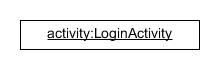
\includegraphics[angle=90,scale = .28]{login_sequenzdiagramm.png}
	       \caption{Login}
	      \end{figure}
	      
	      	\subsection{Ablauf der Methode checkGoogleLoginData()}

Die Methode checkGoogleLoginData() prüft die eingegebenen Google-Login-Daten des Users. Sie wird in der Activity LoginActivity ausgeführt. Als Erstes wird das zugehörige Viewmodel zur Activity, nämlich das LoginViewModel, verwendet. Darauffolgend wird die Methode checkGoogleLoginData(), die in der View-Model-Klasse steht, aufgerufen. In dieser Methode wird der zugehörige Service des Clients, UserService, erstellt, der dann die Verknüpfung zur Server-Seite herstellt. Die Methode getGoogleIdToken des Services wird aufgerufen und als Parameter werden die vom User eingegebenen Login-Daten (E-Mail, Passwort) übergeben. Es wird ein HTTP GET Request an den Google-API-Server gesendet, welcher dann den Google-ID-Token zurücksendet. Der Token wird nun mithilfe der Methode sendGoogleIdToken() an den Server bzw. den zugehörigen UserController gesendet. Im UserController wird die Methode registerOrLogin() aufgerufen. Im UserService des Servers wird ebenfalls eine Methode registerOrLogin() aufgerufen. Das UserRepository ist verantwortlich für die Datenpersistenz und speichert nun also die User-Daten in der Datenbank ab. Auf dem Rückweg zur Activity wird schlussendlich der User übergeben und eine Response gesendet.
	 
	 
		\section{Dynamische Modelle/Erstellen einer Cool Note}
		 \begin{figure}[H]
	       \centering
	       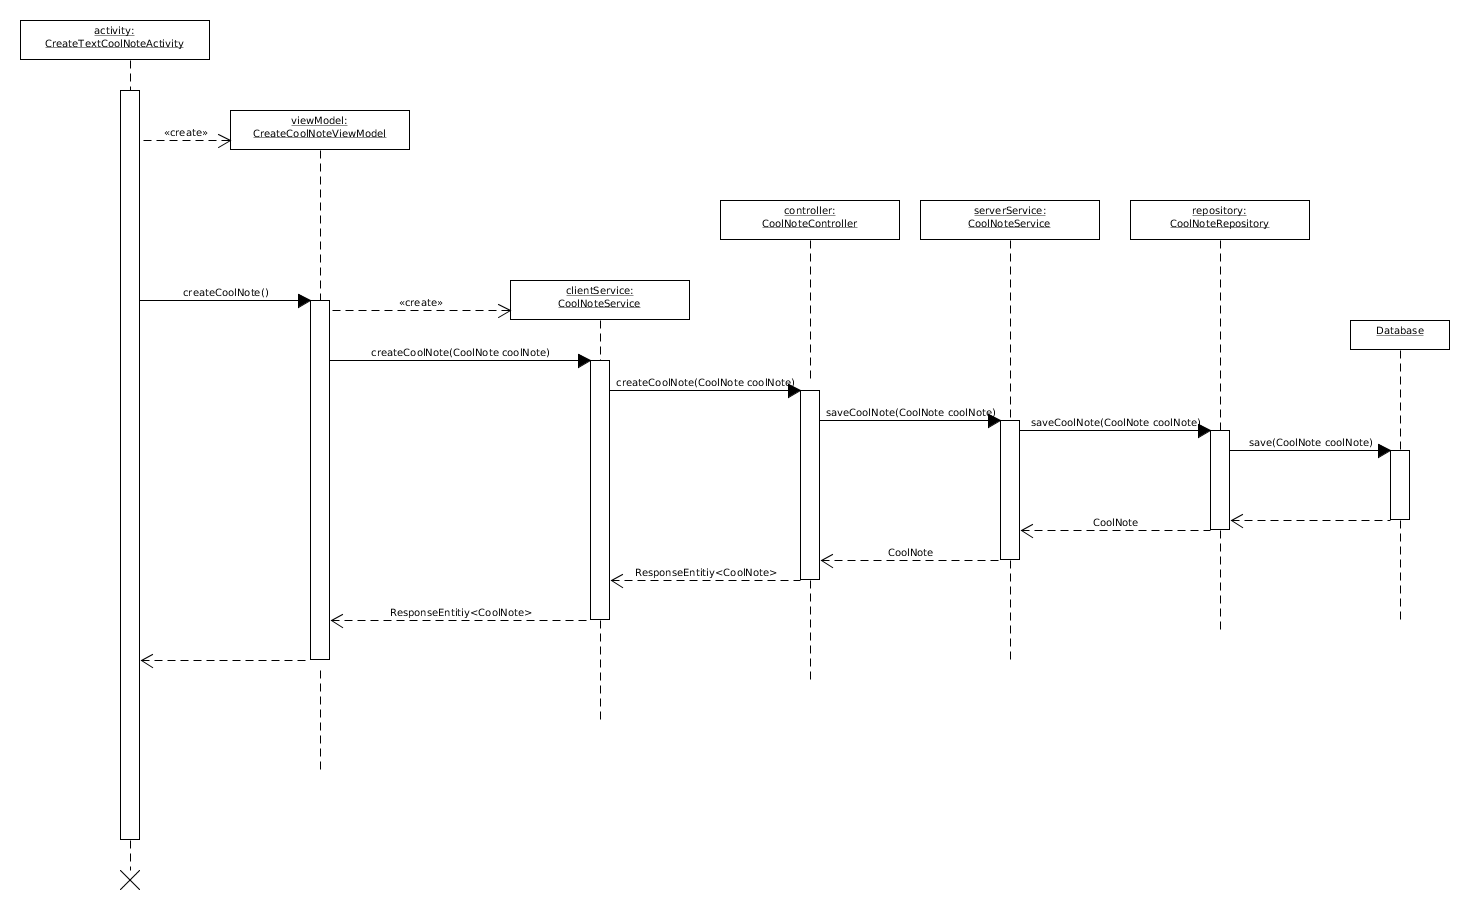
\includegraphics[scale = .35]{SD_CoolNote_erstellen.png}
	       \caption{CoolNote erstellen}
	      \end{figure}
	      
	      
	      	\subsection{Ablauf der Methode createCoolNote()}

Die Methode createCoolNote() erstellt eine Cool Note und platziert sie auf der WG-Pinnwand. Sie wird in diesem Fall in der Activity CreateTextCoolNoteActivity ausgeführt. Als Erstes wird das zugehörige Viewmodel zur Activity, nämlich das CreateCoolNoteViewModel, erstellt bzw. gegettet(?). Darauffolgend wird die Methode createCoolNote(), die in der View-Model-Klasse steht, aufgerufen. In dieser Methode wird der zugehörige Service des Clients, CoolNoteService, erstellt, der dann die Verknüpfung zur Server-Seite herstellt. Die Methode createCoolNote() des Services wird aufgerufen und als Parameter wird eine Instanz des Objektes CoolNote übergeben, welches die vom Benutzer eingetippten Atrribute enthält (Titel, Text-Inhalt, ggfs. Wichtigkeit, Tags, etc.). Der Service schickt ein HTTP POST Request mithilfe des REST-Clients(?) an den Server bzw. an den zugehörigen CoolNoteController. Im CoolNoteController wird die Methode saveCoolNote() aufgerufen, die (irgendwas mit JSON)...? Im CoolNoteService des Servers wird ebenfalls eine Methode saveCoolNote aufgerufen. Das CoolNoteRepository stellt eine Brücke zwischen der Daten und der App dar und speichert nun also die Cool-Note-Daten in der Datenbank ab. Auf dem Rückweg zur Activity wird schlussendlich die erstellte Cool Note übergeben und eine Response gesendet.
		
	      
		\section{Frozen Note bearbeiten}
 	\begin{figure}[H]
	       \centering
	       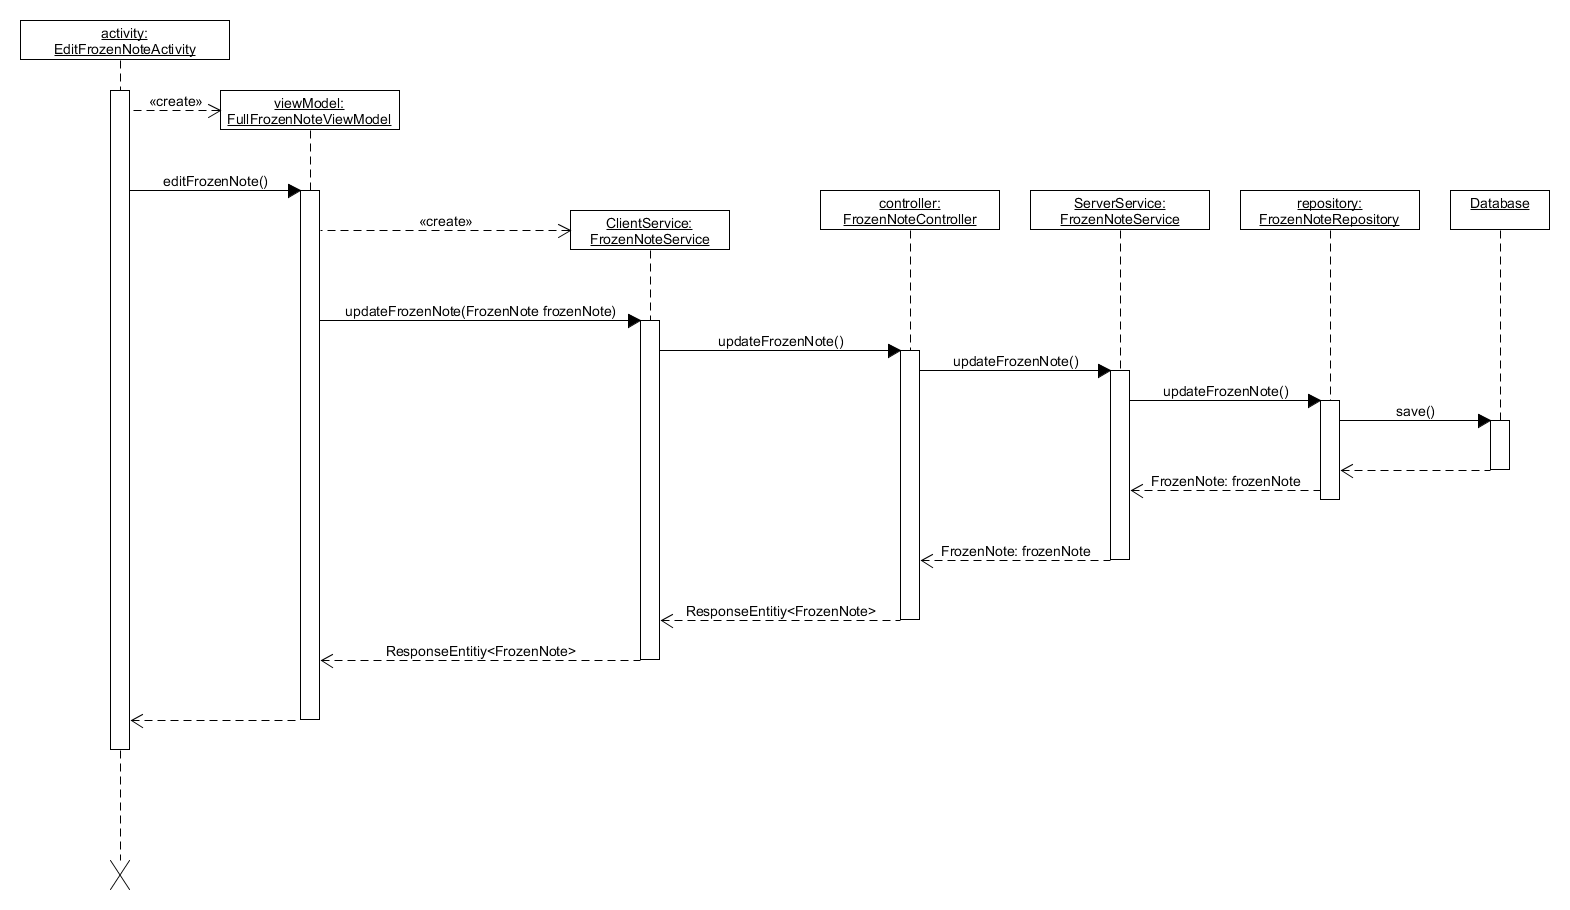
\includegraphics[scale = .35]{Sequenzdiagram_EditFrozenNote.png}
	       \caption{FrozenNote bearbeiten}
	      \end{figure}	
	      
	      \subsection{Ablauf der Methode editFrozenNote()}

Die Methode editFrozenNote() aktualisiert den Inhalt und den Titel einer Frozen Note. Sie wird in der Activity EditFrozenNoteActivity ausgeführt. Als Erstes wird das zugehörige Viewmodel zur Activity, nämlich das FullFrozenNoteViewModel, erstellt bzw. gegettet(?). Darauffolgend wird die Methode editFrozenNote(), die in der View-Model-Klasse steht, aufgerufen. In dieser Methode wird der zugehörige Service des Clients, FrozenNoteService, erstellt, der dann die Verknüpfung zur Server-Seite herstellt. Die Methode updateFrozenNote() des Services wird aufgerufen und als Parameter wird die bereits vorhandene Instanz des Objektes FrozenNote übergeben, welches die vom Benutzer eingetippten Attribute enthält (Titel, Text-Inhalt). Der Service schickt ein HTTP PUT Request mithilfe des REST-Clients(?) an den Server bzw. an den zugehörigen FrozenNoteController. Im FrozenNoteController wird die Methode updateFrozenNote() aufgerufen, die (irgendwas mit JSON)...? Im FrozenNoteService des Servers wird ebenfalls eine Methode updateFrozenNote aufgerufen. Das FrozenNoteRepository stellt eine Brücke zwischen der Daten und der App dar und speichert nun also die neuen Frozen-Note-Daten in der Datenbank ab. Auf dem Rückweg zur Activity wird schlussendlich die editierte Frozen Note übergeben und eine Response gesendet.	
		
		\section{WG verlassen}
		 \begin{figure}[H]
	       \centering
	       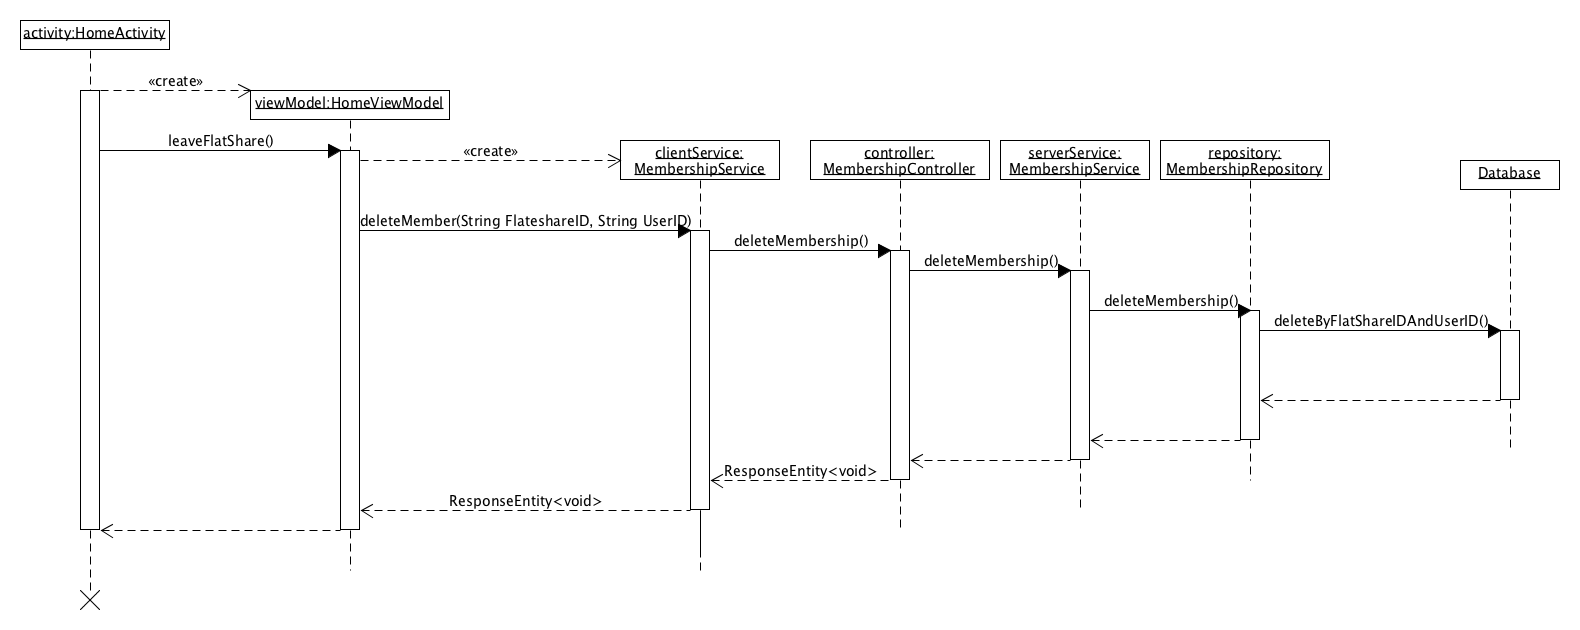
\includegraphics[scale = .35]{SD_WG_verlassen.png}
	       \caption{WG verlassen}
	      \end{figure}
	      	\subsection{Ablauf der Methode leaveFlatShare()}

Die Methode leaveFlatShare() dient zum Verlassen einer WG. Sie wird in der Activity HomeActivity ausgeführt. Als Erstes wird das zugehörige Viewmodel zur Activity, nämlich das HomeViewModel, verwendet. Darauffolgend wird die Methode leaveFlatShare(), die in der View-Model-Klasse steht, aufgerufen. In dieser Methode wird der zugehörige Service des Clients, MembershipService, erstellt, der dann die Verknüpfung zur Server-Seite herstellt. Die Methode deleteMember() des Services wird aufgerufen und als Parameter werden die FlatshareID und die UserID übergeben. Es wird ein HTTP DELETE Request an den Server gesendet bzw. an den zugehörigen Controller. Im MembershipController wird die Methode deleteMembership() aufgerufen. Im FrozenNoteService des Servers wird ebenfalls eine Methode deleteMembership() aufgerufen. Das MembershipRepository ist verantwortlich für die Datenpersistenz und löscht nun also die User-Daten aus der Datenbank. Auf dem Rückweg zur Activity wird schlussendlich eine Response gesendet.
	      

\chapter{Änderungen zum Pflichtenheft}
	\subsection{Kein Archiv}
Wir haben uns dazu entschieden, das Archiv nicht umzusetzen, weil wir andere Wunschkriterien als wichtiger sehen. Außerdem glauben wir, dass Zeitprobleme anfallen würden.

\subsection{Zugangscode-Regelung}
Damit das Zugangscode-Verfahren sicherer ist, haben wir uns dazu entschieden, dass man für jede Einladung einen neuen Zugangscode manuell generieren muss. Dies geschieht dann in der AccessCodeActivity mithilfe eines Buttons. Davor gab es einen dauerhaften Zugangscode für die gesamte WG, nun sind die Zugangscodes einmalig und werden nach der Benutzung  gelöscht. 

\chapter{Glossar}
	\begin{table}[h!]
			\centering
			\label{my-label}
			\begin{tabular}{p{4cm}p{10cm}}
				\textbf{MVVM} & Model View ViewModel  \\
				\textbf{MVC} & Model View Controller  \\
				\textbf{Data Binding} & Automatische Datenweitergabe zwischen Objekten  \\
				\textbf{Client} & User der die App Fridget benutzt   \\
				
				\textbf{Server} &     \\
				\textbf{Activity} & Stellt eine Bildschimrseite in einer App dar   \\
				\textbf{Geschäftslogik} & Mittelschicht einer mehrschichitgen Anwendung  \\
				\textbf{Activity-Lifecycle} Stufen die eine Activity während ihres Lebens durchschreitet   \\
				
				\textbf{API} & Application Programming Interface - Schnittstelle die ein Softwaresystem bereitstellt um dieses in andere Programme einzubinden  \\
				
			
				\textbf{HTTP} & Zustandsloses Protokoll zur Übertragung von Daten auf der Anwendungsschicht über ein Rechnernetz  \\
				\textbf{URL} & Uniform Resource Locator  \\
				\textbf{Open-Source} & Quelltext, welcher öffentlich und von dritten eingesehen, geändert und genutzt werden kann  \\
				
				\textbf{MR-Remote API} &   \\ \todo{RAUS??}
				\textbf{JSON} & JavaScript Object Notation - Datenaustauschformat, das für Menschen einfach zu lesen und für Maschinen einfach zu analysieren und generieren ist   \\
				\textbf{POJO} & Plain Old Java Object  -   \\
				\textbf{Framework} &   \\
				
				\textbf{Instanz} &   \\
				\textbf{Tag / Taggen} &  Markierung und namentliche Erw¨ahnung von Mitgliedern auf Notizzetteln
   \\
				\textbf{Cool-Note} & Notizen, die l¨oschbar, nicht bearbeitbar sind und vom Benutzer erstellt werden   \\
				\textbf{Layout} &   \\
				
				\textbf{Button} & Knopfelement einer Benutzerober߬ache
  \\
				\textbf{Frozen Note} & Notizen, die fest, nicht l¨oschbar, bearbeitbar sind und beim Erstellen der WG generiert werden.
   \\
				\textbf{Nullable} &   \\
				\textbf{NULL} &   \\
				\textbf{Local Repository} &   \\
				\textbf{Parameter} &   \\
				\textbf{Methoden} &   \\
				\textbf{Tutorial} &  Einf¨uhrung in die Funktionen der App
   \\
				\textbf{Check Box} &  Eine Box, die abgehakt werden kann \\
				\textbf{Interface} &   \\
				\textbf{Token} &   \\
				\textbf{Headers} &   \\
				\textbf{Endpoints} &   \\
				\textbf{ResponseEntity} &   \\	
				\textbf{Getter} &   \\	
				\textbf{UUID} &   \\	
				\textbf{ID} &   \\	
				\textbf{Builder} &   \\	
				\textbf{JWT} &   \\	
				\textbf{Repository} &   \\	
				
			\end{tabular}
		\end{table}
	
		


\chapter{Anhang}
\section{Klassendiagramm Client-Server}
 \begin{figure}[H]
	       \centering
	       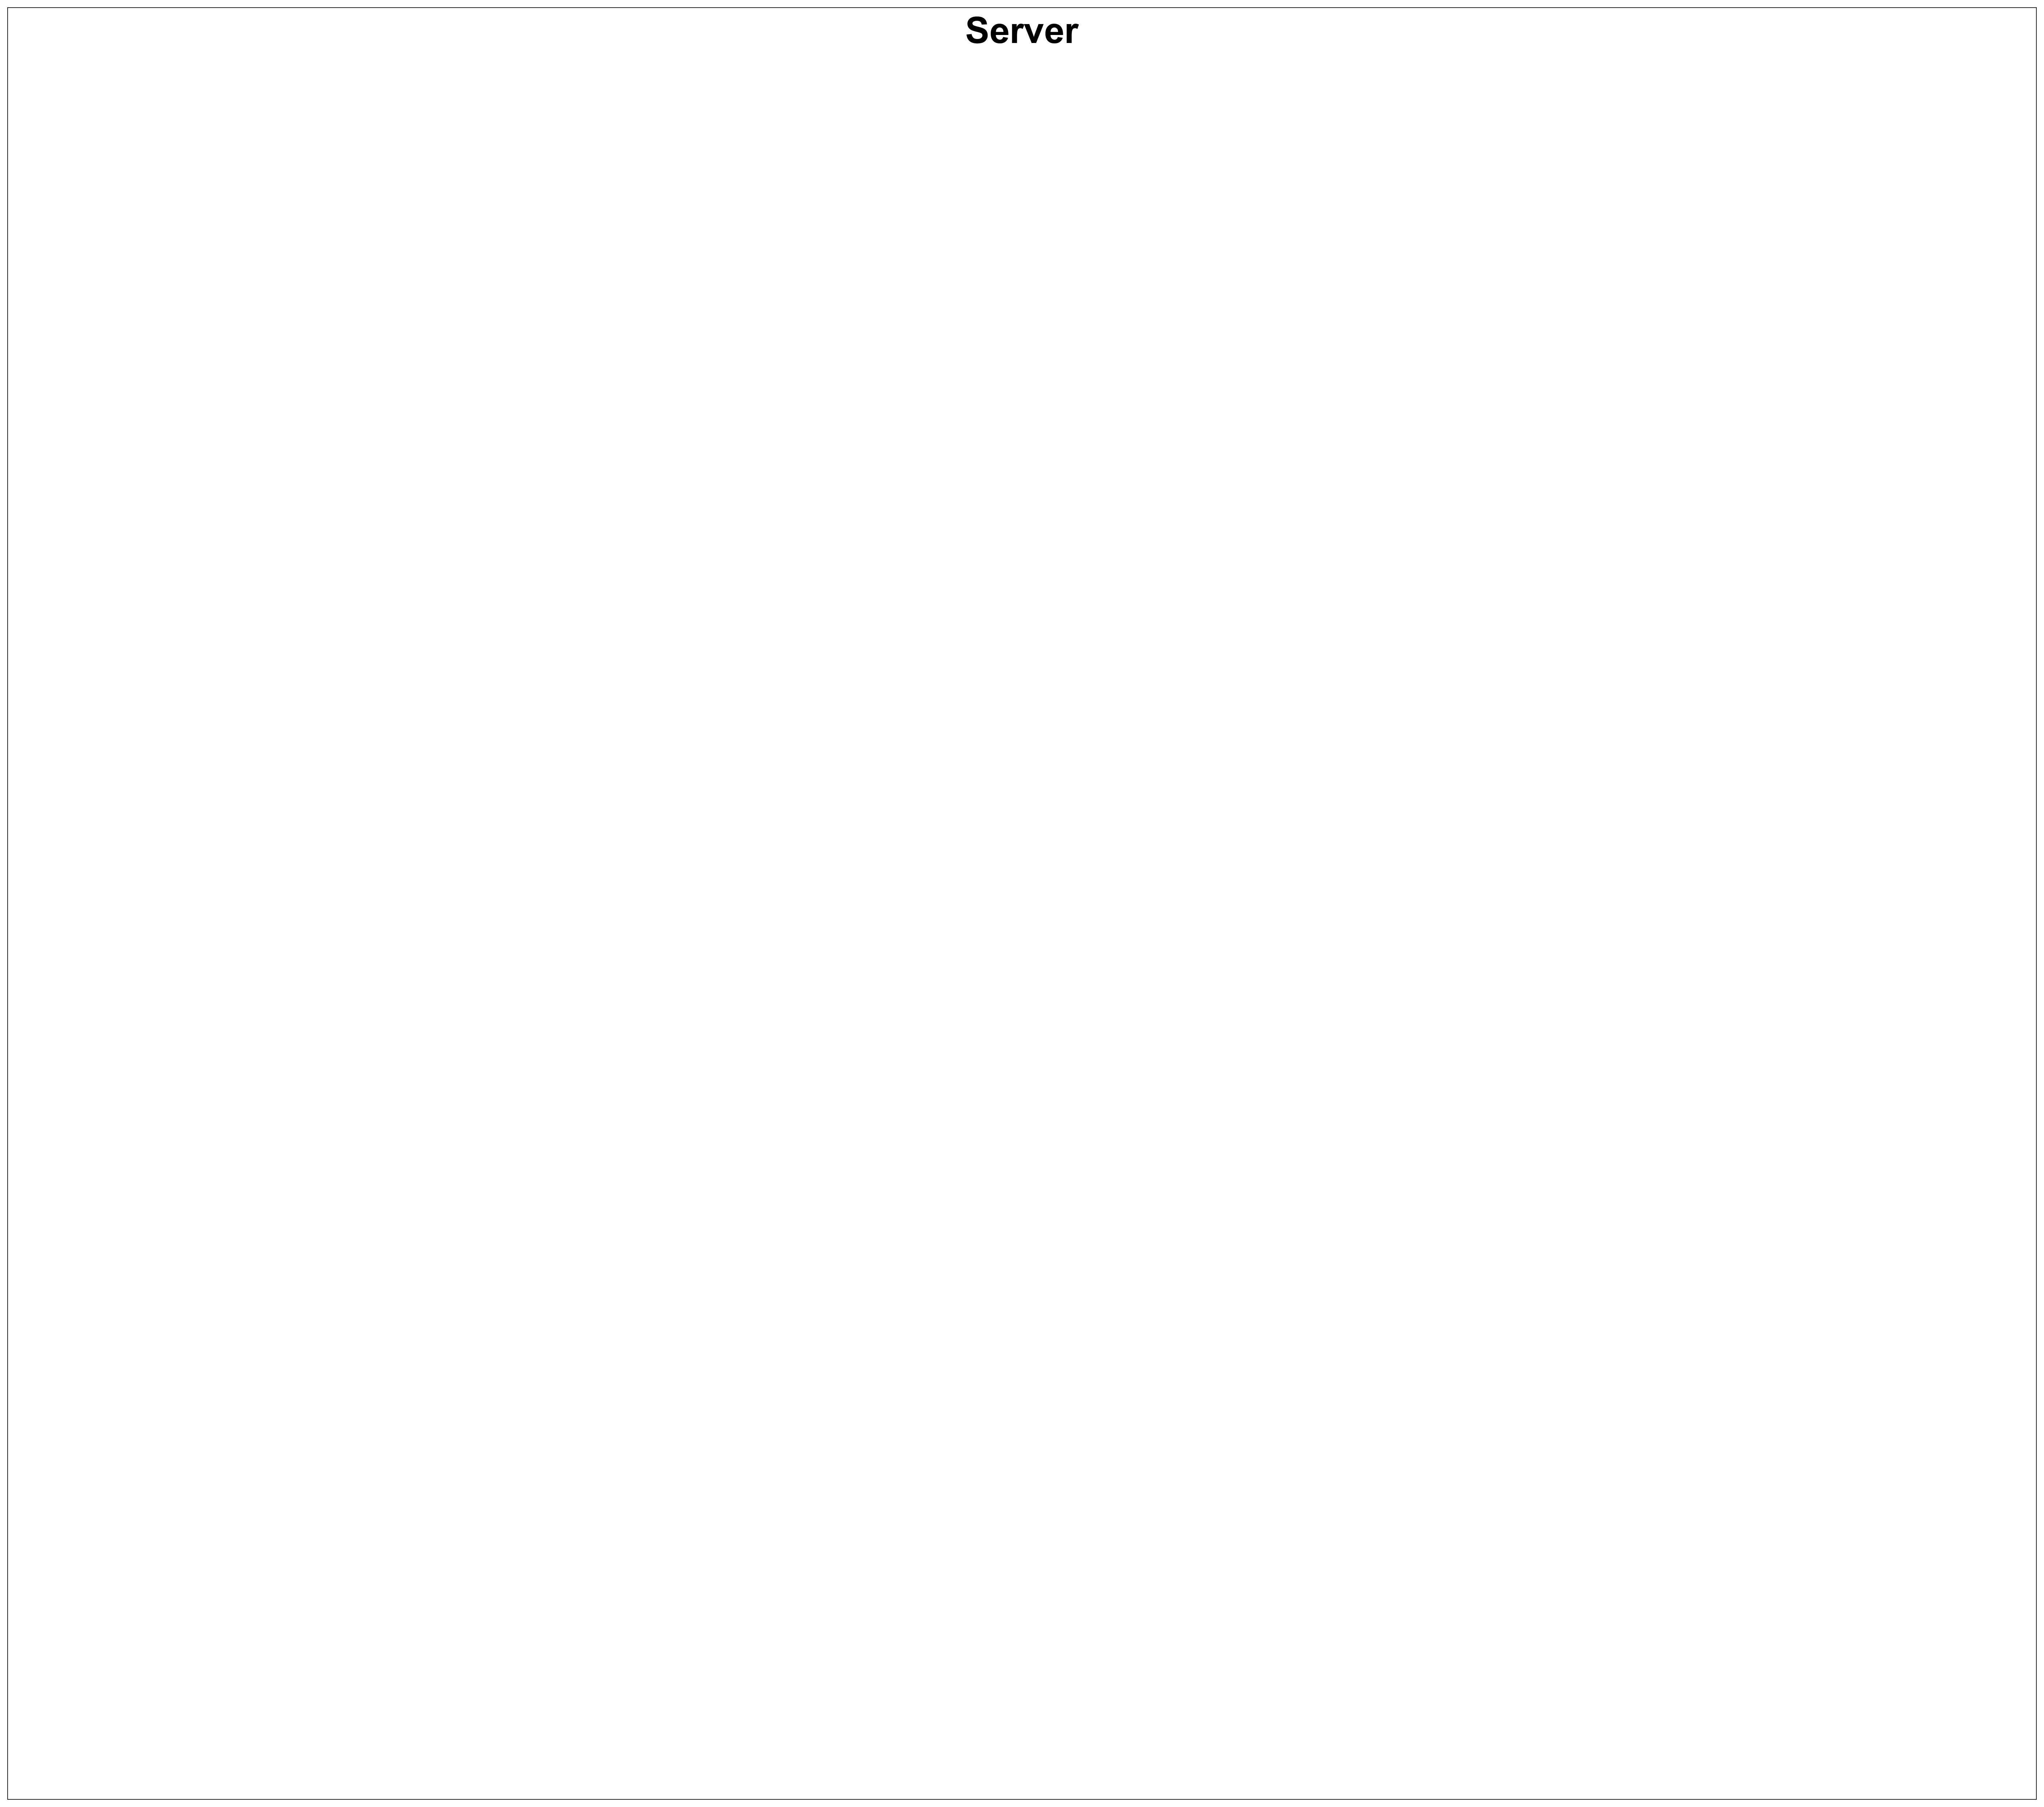
\includegraphics[width=\textwidth,height=\textheight]{client_server_klassen.png}
	       \caption{Client-Server Klassendiagramm}
	      \end{figure}





\end{document}
